% !Rnw root = learnR.Rnw

%% ---preamble.tex----%% 
%% maxwidth is the original width if it is less than linewidth
%% otherwise use linewidth (to make sure the graphics do not exceed the margin)
\makeatletter
\def\maxwidth{ %
  \ifdim\Gin@nat@width>\linewidth
    \linewidth
  \else
    \Gin@nat@width
  \fi
}
\makeatother

\definecolor{fgcolor}{rgb}{0.345, 0.345, 0.345}

\definecolor{shadecolor}{rgb}{.97, .97, .97}
\definecolor{messagecolor}{rgb}{0, 0, 0}
\definecolor{warningcolor}{rgb}{1, 0, 1}
\definecolor{errorcolor}{rgb}{1, 0, 0}






\fbox{\parbox{\textwidth}{{\bf Linear Models, in the style of \txtt{lm()}:}\\[4pt]
\begin{tabular}{ll}
Linear model & Any model that \txtt{lm()} will fit
is a ``linear'' model.\\
& \txtt{lm()} can fit highly non-linear forms of response!\\[6pt]
Diagnostic  & Use \txtt{plot()} with the model object as argument,\\
plots & to get a basic set of diagnostic plots.\\[6pt]
\txtt{termplot()} & If there are no interaction terms,
use \txtt{termplot()}\\
& to visualize the contributions of the different terms.\\[6pt]
Factors & In model formulae, factors model qualitative effects.\\[6pt]
Model & The model matrix shows how coefficients should be\\
 matrices & interpreted. (This is an especial issue for factors.)\\[6pt]
GLMs & Generalized Linear Models are an extension of\\
& linear models, commonly used for analyzing counts.\\[6pt]
Modern &  This can use smoothers -- spline and other functions\\
regession & of explanatory variables that adapt to suit the data.\\[6pt]
GAMs & Generalized Additive Models extend linear models\\
& to allow smoothing curves and surfaces.\\[6pt]
\end{tabular}
\vspace*{3pt}

[NB: \txtt{lm()} assumes independently \& identically distributed (iid)\\
errors, perhaps after applying a weighting function.]
}}
\vspace{12pt}

In this chapter, the chief focus will be on the \txtt{lm()}
(\textit{linear model}) function, discussed earlier in Section
\ref{sec:wr}.  The \txtt{lm()} function is the most widely used of a
huge range of model fitting abilities, available in the various R
packages.

\marginnote[12pt]{Thus spline fits are formed as a linear combination from a
  kitset of curves.}
Linear models are linear in the model parameters, not necessarily in
the variables. A linear model can perfectly well fit a combination of
{\em basis} curves.

\section{Linear Models in R -- Basic Ideas}

Here, we fit a straight line, which is very obviously a linear model!
This simple starting point gives little hint of the range of models
that can be fitted using R's linear model \texttt{lm()} function.

The \texttt{lm()} function returns, as well as estimates, standard
errors for parameters and for predictions. The standard error and
$p$-value information provided by the \txtt{lm()} function assumes
that the random term is i.i.d.\ (independently and identically
distributed) normal.  The independence assumption can be crucial.

The standard errors assume, also, that the analysis is based on a
model was chosen in advance.\sidenote[][-12pt]{The
  standard errors become increasingly unrealistic as the number of
  possible choices of model terms (variables, factors and
  interactions) increases.}  If this is not the case, it can
be important to resort to the use of empirical methods for assessing
model performance -- training/test methodology, or cross-validation,or the bootstrap.

The symbolic notation\sidenote{Wilkinson, GN and Rogers, CE, 1973.
  Symbolic description of models in analysis of variance,
{\em Applied Statistics} 22: 392-399.}  that is available in R for
describing linear models makes it straightforward to set up quite
elaborate and intricate models.

\subsection*{Scatterplot with fitted line -- an example}

The following plots data from the data frame \texttt{roller} (as in
Figure \ref{fig:rollerPlot}) from the \textit{DAAG} package.
\begin{Schunk}
\begin{Sinput}
library(DAAG)
plot(depression ~ weight, data=roller, fg="gray")
\end{Sinput}
\end{Schunk}

\begin{marginfigure}
\begin{Schunk}


\centerline{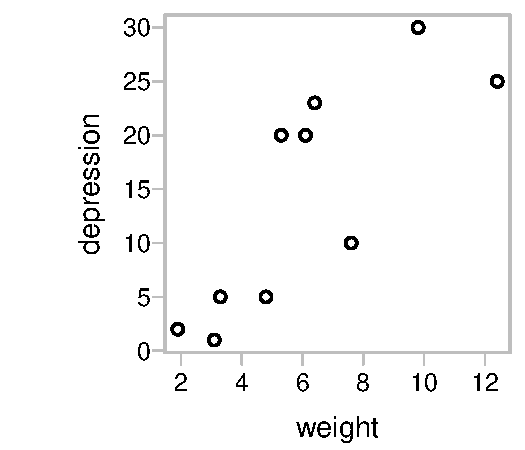
\includegraphics[width=\textwidth]{figs/8-plt-roller-1} }

\end{Schunk}
  \caption{Plot of \txtt{depression} versus \txtt{weight}, using data
from the data frame \txtt{roller} in the {\em DAAG}
package.}\label{fig:rollerPlot}
\end{marginfigure}

The formula \verb!depression ~ weight! can be used either as a
graphics formula or as a model formula. The following
fits a straight line, then adding it to the above plot:
\begin{Schunk}
\begin{Sinput}
plot(depression ~ weight, data=roller, fg="gray")
roller.lm <- lm(depression ~ weight, data=roller)
# For a line through the origin, specify
# depression ~ 0 + weight
abline(roller.lm)
\end{Sinput}
\end{Schunk}
Figure \ref{fig:rollerPlot-withline} repeats the plot, now with a
fitted line added.

\begin{marginfigure}
\begin{Schunk}


\centerline{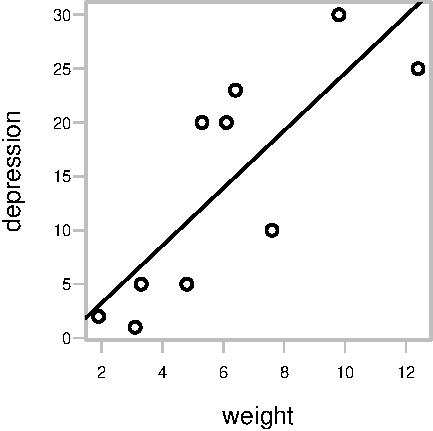
\includegraphics[width=\textwidth]{figs/8-pltWline-1} }

\end{Schunk}
\caption{This repeats Figure \ref{fig:rollerPlot}, now adding a fitted
  line.}\label{fig:rollerPlot-withline}
\end{marginfigure}

The different explanatory variables in the model are called
\texttt{terms}.  In the above, there is one explicit term only on the
right, i.e., \texttt{weight}. This is in addition to the intercept,
which is included by default.

\subsection{Straight line regression -- algebraic details}\label{ss:briefls}
The standard form of simple straight line model can be written\vspace*{-1pt}
\[ \mbox{depression } = \alpha + \beta \times \mbox{ weight } + \mbox{ noise}.
\vspace*{-4pt}
\]
Now write $y$ in place of \texttt{depression} and $x$ in place of
\texttt{weight}, and add subscripts, so that the observations are:
($x_{1}$, $y_{1}$), ($x_{2}$, $y_{2}),\ldots{,} (x_{n}$, $y_{n}$).  Then
the model can be written:
 \[ y_{i} = \alpha + \beta x_{i} + \varepsilon_{i}.\]
The $\alpha +
\beta x_{i}$ term is the ``fixed'' component of the model, and
$\varepsilon_{i}$ is the random noise.

The line is chosen so that the sum of squares of residuals is as small
as possible, i.e., the intercept
$\alpha$ and the slope $\beta$ chosen to minimize
\[ \sum_{i=1}^n (y_i - \alpha - \beta_i x_i)^2 \]

The R function \verb!lm()! will provide estimates $a$ of
$\alpha$ and $b$ of $\beta$. The straight line \vspace*{-2pt}
\[ \widehat{y} = a + b x
\vspace*{-2pt}
\]
can then be added to the scatterplot.

Fitted or predicted values, calculated so that they lie on the
estimated line, are obtained using the formula: \vspace*{-2pt}
\[ \widehat{y}_1 = a + bx_1, \ \widehat{y}_2 = a + bx_2,\ldots{.}
\vspace*{-2pt}
\]
The residuals, which are the differences between the
observed and fitted values, give information about the noise.
\vspace*{-2pt}
\begin{equation}
e_1 = y_1 - \widehat{y}_1, \ e_2 = y_2 - \widehat{y}_2,\ldots{\,.}
\label{e_i}
\end{equation}

\subsection{Syntax -- model, graphics and table formulae:}
The syntax for \texttt{lm()} models that will be demonstrated here is
used, with modification, throughout the modeling functions in R.  A
very similar syntax can be used for specifying graphs and for certain
types of tables.


\subsection*{Model objects}

\marginnote{Components of model objects can be accessed directly, as
  list objects.  But it is usually better to use an extractor
  function. Note in particular \texttt{residuals()} (can be
  abbreviated to \txtt{resid()}), \txtt{coefficients()}
  (\txtt{coef()}), and
  \txtt{fitted.values()} (\txtt{fitted()}).  For example:\\
  \txtt{coef(roller.lm)} }

The following code returns a model object to the command line.
\begin{Schunk}
\begin{Sinput}
lm(depression ~ weight, data=roller)
\end{Sinput}
\begin{Soutput}

Call:
lm(formula = depression ~ weight, data = roller)

Coefficients:
(Intercept)       weight  
      -2.09         2.67  
\end{Soutput}
\end{Schunk}
\noindent
When returned to the command line in this way,
a printed summary is returned.  

Alternatively, the result can be saved as a named object,
which is a form of list.
\begin{Schunk}
\begin{Sinput}
roller.lm <- lm(depression ~ weight, data=roller)
\end{Sinput}
\end{Schunk}

The names of the list elements are:
\begin{Schunk}
\begin{Sinput}
names(roller.lm)
\end{Sinput}
\begin{Soutput}
 [1] "coefficients"  "residuals"     "effects"       "rank"         
 [5] "fitted.values" "assign"        "qr"            "df.residual"  
 [9] "xlevels"       "call"          "terms"         "model"        
\end{Soutput}
\end{Schunk}

\subsection{Matrix algebra -- straight line regression example}
In order to write the quantity
\[\sum_{i=1}^{10} (y_i - a - b x_i)^2\]
that is to be minimized in matrix form, set:
\begin{fullwidth}
\begin{minipage}[c]{0.25\textwidth}
\[
\mathbf{X} = \left( \begin{array}{cc}
  1 & 1.9\\
  1 & 3.1\\
  1 & 3.3\\
  1 & 4.8\\
  1 & 5.3\\
  1 & 6.1\\
  1 & 6.4\\
  1 & 7.6\\
  1 & 9.8\\
  1 & 12.4
\end{array} \right)
\]
    \end{minipage}
\begin{minipage}[c]{0.015\textwidth}
\[\mathbf{;}\]
\end{minipage}
\hspace{0.025\textwidth}
    \begin{minipage}[c]{0.18\textwidth}
\[
\mathbf{y} = \left( \begin{array}{c}
  2\\
  1\\
  5\\
  5\\
 20\\
 20\\
 23\\
 10\\
 30\\
 25
\end{array} \right)
\]
    \end{minipage}
    \begin{minipage}[c]{0.015\textwidth}
\[\mathbf{;}\]
\end{minipage}\hspace{0.05\textwidth}
\begin{minipage}[c]{0.44\textwidth}
\[\mathbf{e} = \mathbf{y} - \mathbf{X} \mathbf{b} =
\left( \begin{array}{c}
  2  - (a + 1.9 b)\\
  1  - (a + 3.1 b)\\
  5  - (a + 3.3 b)\\
  5  - (a + 4.8 b)\\
 20  - (a + 5.3 b)\\
 20  - (a + 6.1 b)\\
 23  - (a + 6.4 b)\\
 10  - (a + 7.6 b)\\
 30  - (a + 9.8 b)\\
 25  - (a + 12.4 b)
\end{array} \right)
\]
\end{minipage}\hspace{0.1\textwidth}
    \begin{minipage}[c]{0.36\textwidth}
\[\mbox{where}\;\;\; \mathbf{b} =
\left( \begin{array}{c}
a\\
b
\end{array} \right)
\]
\end{minipage}\vspace*{0.025\textwidth}
\end{fullwidth}

Here $a$ and $b$ are chosen to minimize the sum of squares of elements
of $  \mathbf{e} = \mathbf{y} - \mathbf{X} \mathbf{b}$, i.e., to
minimize
\[ \mathbf{e}'\mathbf{e} = (\mathbf{y} - \mathbf{X} \mathbf{b})'
(\mathbf{y} - \mathbf{X} \mathbf{b})
\]
The least squares equations can be solved using matrix arithmetic.

\subsection*{Recap, and Next Steps in Linear Modeling}
For this very simple model, the model matrix had two columns
only.  Omission of the intercept term will give an even simpler model
matrix, with just one column.

Regression calculations in which there are several explanatory variables
are handled in the obvious way, by adding further columns as necessary to
the model matrix.  This is however just the start to the rich range of
possibilities that model matrices open up.

\subsection{A note on the least squares methodology}\label{ss:lsAssume}

\marginnote[12pt]{The assumptions of independence and identical
distribution (iid) are crucial. The role of normality is commonly
over-stated.}
More fundamental than least squares is the maximum likelihood
principle.  If the ``error'' terms are independently and identically
normally distributed, then least squares and maximum likelihood are
equivalent.

Least squares will not in general yield maximum likelihood estimates,
and the SEs returned by \texttt{lm()} or by \texttt{predict()} from
an \texttt{lm} model will be problematic or wrong if:
\begin{itemize}
\item Variances are not homogeneous\sidenote{Weighted least squares is
    however justified by maximum likelihood if it is known how the
    variances change with $x_i$, or if the pattern of change can be
    inferred with some reasonable confidence.};
    \item Observations are not independent;
    \item The sampling distributions of parameter estimates are
      noticeably non-normal.
    \item Model terms 
\marginnote{Simplifying the model, in ways that do not much
affect coefficients that remain in the model, may be acceptable.}
    (variables, factors and/or interactions) have
      been chosen from some wider set of possibilities (the theory
      assumes a specfic known model).
 \end{itemize}

 Normality of the model 'errors' is more than is in practice required.
 Outliers, and skewness in the distribution, do often mean that the
 theory cannot be satisfactorily used as a good approxation.

\section{Checks --- Before and After Fitting a Line}

Consider here a female versus male comparison of record times for
Northern Island hill races.

\paragraph{Untransformed vs transformed scales:}

\begin{figure}
\begin{Schunk}


\centerline{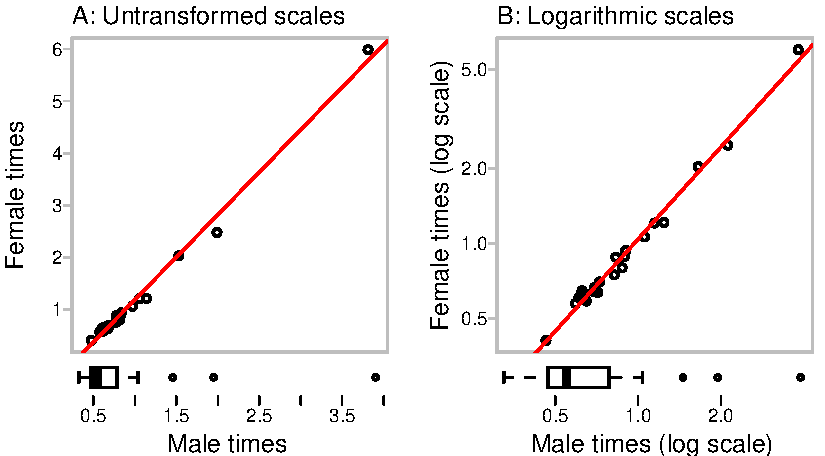
\includegraphics[width=\textwidth]{figs/8-fVSmTimeAB-1} }

\end{Schunk}
  \caption{Graphs compare female with male record times,
  for Northern Ireland hill races.  Least squares lines
    are added, and marginal boxplots are shown on the
    horizontal axis. Panel A
    has untransformed scales, while Panel B has log
    transformed scales. For the code, see the script
    file for this chapter.}\label{fig:nimff}
\setfloatalignment{t}% forces caption to be top-aligned
\end{figure}

Figure \ref{fig:nimff} shows two alternative views of the data.
Least squares line have in each case been added.  

In Panel A, a single data point at the top right lies well
away from the main body of data.  In Panel B, points are more
evenly spread out, though still with a tail out to long times.

The following fits a regression line on the untransformed
scale:
\begin{Schunk}
\begin{Sinput}
mftime.lm <- lm(timef ~ time, data=nihills)
\end{Sinput}
\end{Schunk}

The line appears to fit the data quite reasonably well. Is this an
effective way to represent the relationship?  An obvious problem is
that data values become increasingly sparse as
values increase, with one point widely separated from other data.
That one data point, widely separated from other points, stands
to have a disproportionate effect in determining the fitted line.

The coefficients for the line that is fitted on a logarithmic
scale is:
\begin{Schunk}
\begin{Sinput}
mflogtime.lm <- lm(log(timef) ~ log(time),
                   data=nihills)
round(coef(mflogtime.lm), 3)
\end{Sinput}
\begin{Soutput}
(Intercept)   log(time) 
      0.267       1.042 
\end{Soutput}
\end{Schunk}
The coefficient of 1.042 for \txtt{log(time)} implies that the
relative rate of increase of female times is 4.2\% greater than the
relative rate of increase of male times.

\subsection*{The use of residuals for checking the fitted line:}
In Figure \ref{fig:nimff}, departures from the line do not stand out
well relative to the line.  To make residuals stand out, Figures
\ref{fig:to-horiz}A and \ref{fig:to-horiz}B rotate the lines, for the
untransformed and transformed data respectively, $\sim$45$^{\circ}$
clockwise about its mid-point, to the horizontal.

\begin{figure}
\begin{Schunk}


\centerline{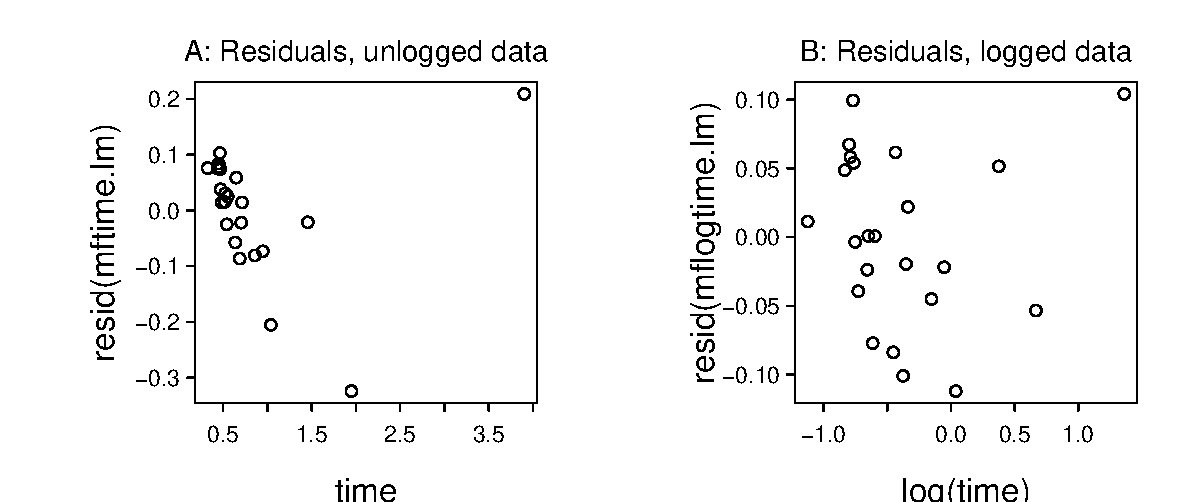
\includegraphics[width=\textwidth]{figs/8-tohoriz-mf-1} }

\end{Schunk}
\caption{In Panel A, residuals from the line for the unlogged data
  have been plotted against male times.  Panel B repeats the same
  type of plot, now for the regression for the logged data.\label{fig:to-horiz}}
\end{figure}

\noindent
Notice that, in Figure \ref{fig:to-horiz}A, all residuals except that
for the largest time lie very nearly on a line.  The point with the
largest fitted value, with the largest male (and female) time, is
pulling the line out of whack.  There is a mismatch between the data
and the model.  The picture in Figure \ref{fig:to-horiz}B is much
improved, though there still is an issue with the point for the
longest time.

\marginnote[12pt]{A residual of -0.1 denotes a
time that is about 10\% (more accurately 9.5\%) less than the fitted
value on the line.  A residual of 0.1 denotes a time that is about
10\% (more accurately 10.5\%) more than the fitted value.}
Residuals on the vertical scale of Figure \ref{fig:to-horiz}B are on a
scale of natural logarithms (logarithms to base $e$).  As the range is
small (roughly between -0.1 and 0.1), the values can be interpreted as relative
differences on the scale of times.


\paragraph{The common benefits of a logarithmic transformation:}

Where measurement data have a long tail out to the right, it
commonly makes sense to work with logarithms of data values, as in Figure
\ref{fig:nimff}B.  Often, working with data on a logarithmic
scale has several useful consequences:
\begin{itemize}
  \item[-] The skewness is reduced
  \item[-] The variation at the high end of the range of values is reduced,
    relative to variation at the low end of the range of values.
  \item[-] Working on a logarithmic scale is equivalent to working
    with relative, rather than absolute, change.  Thus a change from
    10 to 20 is equivalent to a change from 20 to 40, or from 40 to 80.
    On a logarithmic scale, these are all changes by an amount of
    $\log(2)$.
  \item[-] By default, the function \txtt{log()}) returns natural
    logarithms, i.e., logarithms to base $e$.  On this scale, a change
    of 0.05 is very close to a change of 5\%.  A change of 0.15 is
    very roughly a change of 15\%.  [A decrease of 0.15 is a decrease
    of $\simeq 13.9\%$, while an increase of 0.15 is a increase of
    $\simeq 16.2\%$]
\end{itemize}

Once the model is fitted, checks can and should be made on the extent
and manner of differences between observations and fitted model
values.  Graphical checks are the most effective,\sidenote{Statistics
  that try to provide an overall evaluation focus too much on a
  specific form of departure, and do a poor job at indicating whether
  the departure from assumptions matters.} at least as a starting
point. Mostly, such checks are designed to highlight common types of
departure from the model.

Figure \ref{fig:to-horiz}B provided a simple form of diagnostic check.
This is one of several checks that are desirable when models
have been fitted.

\subsection{$^*$Diagnostics -- checks on the fitted model}\label{ss:diag}

\marginnote{Section \ref{sec:simcheck} demonstrates the use of
  simulation to help in judging between
genuine indications of model departures and features of the plots that
may well reflect statistical variation.}
For \texttt{lm} models, the R system has a standard set of diagnostic
plots that users are encouraged to examine.  These are a starting
point for investigation. Are apparent departures real, or may they be a
result of statistical variation?  For the intended use of the model
output, do apparent departures from model assumptions matter.

For drawing attention to differences between the data and what might
be expected given the model, plots that show residuals are in general
much more effective than plots that show outcome ($y$) variable
values. Additionally, plots are needed that focus on common specific
types of departure from the model.

\subsection*{All four diagnostic plots}
Figure \ref{fig:diag-mftime} shows the default
diagnostic plots for the regression with the untransformed data:

\begin{figure*}
\begin{Schunk}


\centerline{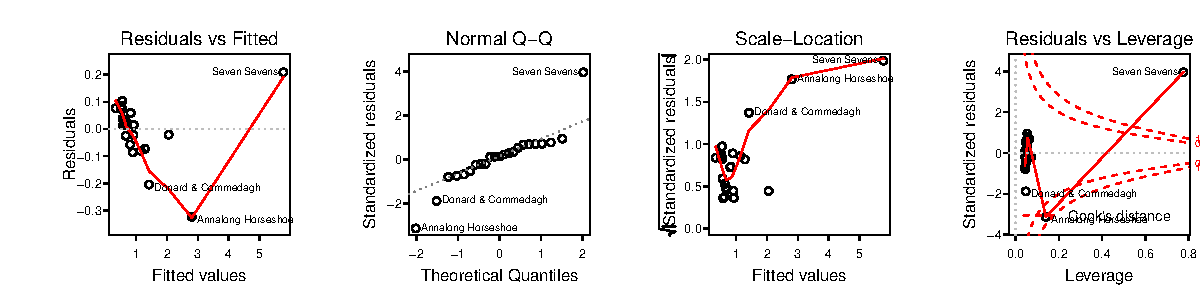
\includegraphics[width=\textwidth]{figs/8-diag-mf-1} }

\end{Schunk}
\caption{Diagnostic plots from the regession of \txtt{timef} on
  \txtt{time}.}\label{fig:diag-mftime}
\end{figure*}
\noindent
Simplified code is:
\begin{Schunk}
\begin{Sinput}
mftime.lm <- lm(timef ~ time, data=nihills)
plot(mftime.lm, cex.caption=0.8)
\end{Sinput}
\end{Schunk}
The first of these plots has similar information to Figure \ref{fig:to-horiz}A
above.  A difference is that residuals are now plotted against fitted
values.  It is immaterial, where there is just one explanatory variable,
whether residuals are plotted against fitted values or against
$x$-values -- the difference between plotting against $a + b x$ and
plotting against $x$ amounts only to a change of labeling on the
$x$-axis.

\marginnote{Two further plots are available; specify \margtt{which=4}
or \margtt{which=6}, e.g.\\
\margtt{plot(mftime.lm, which=4}.  These give a different slant
on what is shown in the fourth default plot (\margtt{which=5}).}
Figure \ref{fig:diag-mftime-log} shows the default
diagnostic plots for the transformed data.
Simplified code is:
\begin{Schunk}
\begin{Sinput}
plot(mflogtime.lm, cex.caption=0.8)
par(opar)
\end{Sinput}
\end{Schunk}
\begin{figure*}
\begin{Schunk}


\centerline{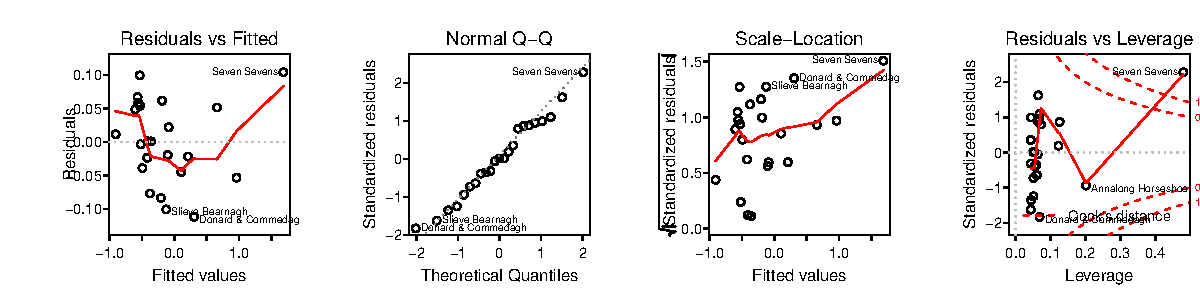
\includegraphics[width=\textwidth]{figs/8-diag-logmf-1} }

\end{Schunk}
\caption{Diagnostic plots from the regression of \txtt{log(timef)} on
  \txtt{log(time)}.}\label{fig:diag-mftime-log}
\end{figure*}
\noindent
The point for the largest
time still has a very large leverage and, as indicated by its position
relative to the Cook's distance contours, a large influence on the
fitted regression line.  This may, in part or entirely, be a result of
a variance that, as suggested by the scale-location plot in Panel 3,
tends to increase with increasing fitted value.  The normal Q-Q plot
(Panel 2) suggests an overall distribution of residuals that is
acceptably normal.  The large residual associated with the largest
time in Panel 1 would look much less out of place if there was an
adjustment that allowed for a variance that increases with increasing
fitted value.

These differences from the assumed model are small enough that, for
many purposes, the line serves as a good summary of the data.  The
equation is:
\begin{Schunk}
\begin{Sinput}
mflogtime.lm <- lm(log(timef) ~ log(time),
                   data=nihills)
round(coef(mflogtime.lm), 3)
\end{Sinput}
\begin{Soutput}
(Intercept)   log(time) 
      0.267       1.042 
\end{Soutput}
\end{Schunk}
The coefficient that equals 1.042 can be interpreted as a relative rate of
increase, for female time relative to male time. Consider a race
for which the male record time is 100 minutes.  The predicted female
time is:
\[
\mbox{exp}(0.267 + 1.042 \log(100/60))
= 2.223\mbox{h}
= 133.4\mbox{m}.
\]
An increase of one minute, or 1\%, in the male time, is predicted to lead
to an increase of close to 1.042 $\times$ 1\% in the
female time.  The predicted increase is 133.4 $\times$ 1.042m.

\paragraph{Panel 2 --- A check for normality:}
\begin{marginfigure}[1.0cm]
To obtain this second plot only, without the others, type:
\begin{Schunk}
\begin{Sinput}
plot(mftime.lm, which=2)
\end{Sinput}
\end{Schunk}
\end{marginfigure}
The second panel in Figure
\ref{fig:diag-mftime} identifies two large negative residuals and one
large positive residual.  This seems inconsistent with the assumption
that residuals have a normal dsitribution.  Again, Figure
\ref{fig:diag-mftime-log} shows an improvement.

Modest departures from normality are not a problem per
se. Heterogeneity of variance, and outliers in the data, are likely to
be the more serious issues.

\paragraph{Panel 3 --- Is the variance constant?:}
\begin{marginfigure}[1.0cm]
 To obtain this third plot only, without the others, type:
\begin{Schunk}
\begin{Sinput}
plot(mftime.lm, which=3)
\end{Sinput}
\end{Schunk}
\end{marginfigure}
The third panel is designed to check whether variation about the
fitted line, as measured by the variance, is constant.  For this,
there should be no trend up or down in the points.  The large
upward trend in the third panel of
\ref{fig:diag-mftime} has largely disappeared in the third panel
of Figure \ref{fig:diag-mftime-log}.

\paragraph{Panel 4 --- a check for high leverage points:}
\begin{marginfigure}[1.0cm]
 To obtain this fourth plot only, without the others, type:
\begin{Schunk}
\begin{Sinput}
plot(mftime.lm, which=5)
\end{Sinput}
\end{Schunk}
\end{marginfigure}
The fourth panel is designed to check on points with
large leverage and/or large influence.  In straight line regression,
the most extreme leverage points are points that are separated from
the main body of points, and are at the high or (less commonly) low
end of the range of $x$-values.

The combined
\marginnote{For working within the main range of the data values, we
  might prefer to use the regression line that is obtained when `Seven
  Sevens' is omitted. If `Seven Sevens' is omitted in estimating the
  regression line, this should be made clear in any report, and the
  reason explained.  The large residual for this point does hint that
  extrapolation much beyond the upper range of data values is
  hazardous.}
effect of leverage and magnitude of residual determines
what {\em influence} a point has.  Large leverage translates into
large influence, as shown by a large Cook's distance, when the
residual is also large.  Points that lie within the region marked out
by the 0.5 or (especially) the 1.0 contour for Cook's distance have a
noticeable influence on the fitted regression equation.  Even with the
logged data, the point for the largest time (`Seven Sevens') is
skewing the regression line noticeably.

Note that there is no reason to suspect any error in this value.  Possibly
the point is taking us into a part of the range where the relationship
is no longer quite linear.  Or this race may be untypical for more
reasons than that it is an unusually long race.

The following shows the change when `Seven Sevens' is omitted:
\begin{Schunk}
\begin{Sinput}
round(coef(mflogtime.lm), 4)
\end{Sinput}
\begin{Soutput}
(Intercept)   log(time) 
     0.2667      1.0417 
\end{Soutput}
\begin{Sinput}
omitrow <- rownames(nihills)!="Seven Sevens"
update(mflogtime.lm, data=subset(nihills, omitrow))
\end{Sinput}
\begin{Soutput}

Call:
lm(formula = log(timef) ~ log(time), data = subset(nihills, omitrow))

Coefficients:
(Intercept)    log(time)  
      0.239        0.991  
\end{Soutput}
\end{Schunk}

 \subsection{The independence assumption is crucial}

 A key assumption is that observations are independent.  The
 independence assumption is an assumption about the process that
 generated the data, about the way that it should be modeled.
 There is no one standard check that is relevant in all circumstances.
 Rather the question should be: ``Are there aspects of the way that
 the data were generated that might lead to some form of dependence?''
 Thus, when data are collected over time, there may be a time series
 correlation between points that are close together in time.

 Another possibility is some kind of clustering in the data, where
 observations in the same cluster are correlated. In medical
 applications, it is common to have multiple observations on the one
 individual.   Where clusters may be present, but there is no way to
 identify them, dependence is hard or impossible to detect.

 Issues of dependence can arise in an engineering maintenance context.
 If the same mechanic services two aircraft engines at the same time
 using replacement parts from the same batch, this greatly increases
 the chances that the same mistake will be made on the two engines, or
 the same faulty part used.  Maintenance faults are then not
 independent. Independence is not the harmless assumption that it is
 often made out to be!

There may be further checks and tests that should be applied.
These may be specific to the particular model.

\section{$^*$Simulation Based Checks}\label{sec:simcheck}

\marginnote{If the assumption of independent random errors is wrong,
  patterns in the diagnostic plots that call for an explanation
  may be more common than suggested by the simulations.}
A good way to check whether indications of departures from the model
may be a result or random variation is to compare the plot with
similar plots for several sets of simulated data values, as a means
of verifying that the mismatch is, if residuals from the line are
independent and normally distributed, real. This is the motivation
for Figure \ref{fig:4sim-mftimeres1}. 
  

\begin{figure}
\vspace*{-12pt}

\begin{Schunk}


\centerline{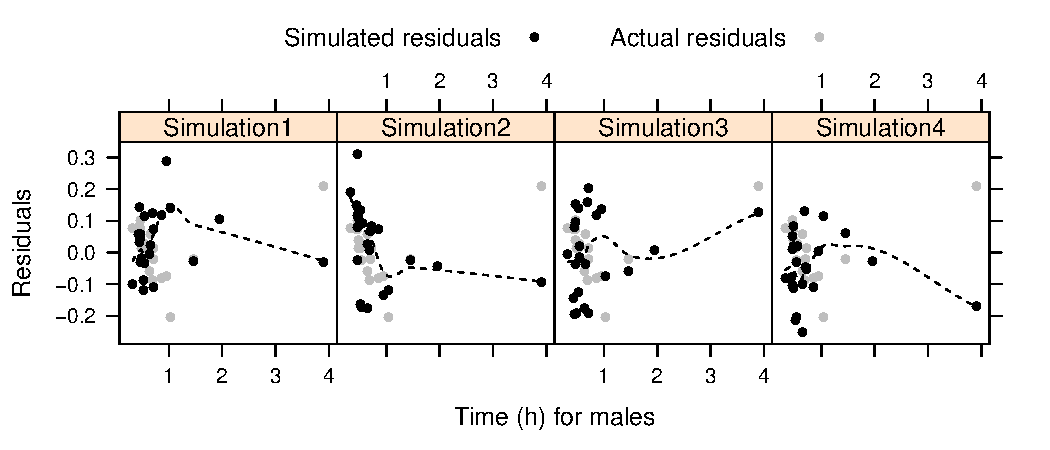
\includegraphics[width=\textwidth]{figs/8-simscat-1} }

\end{Schunk}
\caption{The plots are four simulations of residuals, from the
  model that is fitted to the unlogged data.  The coefficients
  used, and the standard deviation, are from the fitted least squares
  line.\label{fig:4sim-mftimeres1}}
\setfloatalignment{b}%
\end{figure}
\begin{Schunk}
\begin{Sinput}
## Code
gph <- plotSimScat(obj=mftime.lm, show="residuals",
                   type=c("p","smooth"),
                   layout=c(4,1))
update(gph, xlab="Time (h) for males",
      ylab="Residuals")
\end{Sinput}
\end{Schunk}

The simulations indicate that there can be a pattern in the smooth
curve that is largely due to the one point that is widely separated
from other data. On the other hand, the very large residual seen in
the actual data is not matched in any of the simulations.

This type of check can be repeated for the other diagnostic plots:
\begin{itemize}
  \item [-] A check for normality (Panel 2: \txtt{which=2}.  Type:
\begin{Schunk}
\begin{Sinput}
plotSimDiags(obj=mftime.lm, which=2, layout=c(4,1))
\end{Sinput}
\end{Schunk}
\item[-] Is the variance constant? (Panel 3: \txtt{which=3}.  Type:
\begin{Schunk}
\begin{Sinput}
plotSimDiags(obj=mftime.lm, which=3, layout=c(4,1))
\end{Sinput}
\end{Schunk}
\item[-]  Are there issues of leverage and influence? (Panel 4:
  \txtt{which=5}.  Type:
\begin{Schunk}
\begin{Sinput}
plotSimDiags(obj=mftime.lm, which=5, layout=c(4,1))
\end{Sinput}
\end{Schunk}
\end{itemize}

\subsection*{Scatterplots that are derived from the simulation process}

To see scatterplots that are derived from the simulation process,
use the function \txtt{plotsimscat()}, from the {\em DAAG} package.
For example, try, working with the untransformed data:
\begin{Schunk}
\begin{Sinput}
gph <- plotSimScat(mftime.lm, layout=c(4,1))
update(gph, xlab="Male record times (h)",
       ylab="Female record times (h)")
\end{Sinput}
\end{Schunk}
Observe that the largest simulated value lies consistently above the
data value. Other simulated values, for male times of more than around
one hour, tend to lie below the actual data.  This is much easier to
see in the plots of residuals.  A scatterplot that shows the actual
data values is not a good tool for making these difference
visually obvious.

 \section{Key questions for the use of models}

Key questions are:
\begin{itemize}
\item Modeling and analysis
  \begin{itemize}
    \item Which model?
    \item Do we want to make predictions?  Or is the interest in getting
parameter estimates that are interpretable?
    \item How will model performance be measured?
    \item How close can we get to measuring the performance that matters?
  \end{itemize}
\item Interpretation
  \begin{itemize}
    \item The task is easier if the aim is prediction, rather than
interpretation of model parameters.
    \item Can model parameters be interpreted in scientifically meaningful
      ways?\newline
      [This is a minefield, with huge scope for getting it wrong.]
  \end{itemize}
\end{itemize}

More detailed comments will now follow on some of the issues raised above.

\paragraph{The choice of  method:} Note the use of the word ``method'',
not algorithm. Algorithms specify a sequence of computational steps.
Something more than an algorithm is needed, if results are to have
some use that generalizes beyond the specific data used.

There are many different methods. How should the analyst
choose between them?  What are good ways to assess the performance of
one or other algorithm? A credible measure of model performance is
needed, evaluated on test data that closely reflects the context in
which the model will be applied.

\paragraph{Which are the important variables?} Often, the analyst
would like to know which data columns (variables, or features) were
important for, e.g., a classification.  Could some of them be omitted
without loss?

The analyst may wish to attach an interpretation to one or more
coefficients?  Does the risk of heart attack increase with the amount
that a person smokes?  For a meaningful interpretation of model
parameters, it is necessary to be sure that:
\begin{itemize}
\item All major variables or factors that affect the outcome have been
  accounted for.
\item Those variables and factors operate, at least to a first
order of approximation, independently.
\end{itemize}

In some cases, a different but equivalent choice of parameters will be
more meaningful.  For working with the Northern Ireland hillrace data
in Subsection \ref{sec:nihills-reg}, the parameters \texttt{dist} and
\texttt{climb} clearly do not exercise their effects independently,
making their coefficients difficult to interpret. It is better to work
with \texttt{log(dist)} and \texttt{log(dist/climb)}, which are very
nearly independent.

See Rosenbaum's {\em Observational Studies}\sidenote{{Rosenbaum, P.R},
    2002.  \textit{Observational Studies}, 2nd edn.
    Springer-Verlag.} for comments on approaches
that are often useful in the attempt to give meaningful
interpretations to coefficients that are derived from observational
data.

\section{Factor Terms -- Contrasts}\label{ss:facs}

Here,\marginnote[-30pt]{Another special type of term is one that allows
  smooth functions of explanatory variables.  Again, linear models can
  be adapted to handle such terms.} we show how regression models can
be adapted to fit terms involving factors.

\begin{table}[h]
\tabcolsep12pt
%\begin{center}
\begin{tabular}{@{}llll@{}}
    Water & A  & B  & C  \\
 (Water only) & (Additive 1) & (Additive 2) & (Additive 3)\\
\hphantom{Mean $=$} 1.50 & 1.50  &1.90 &1.00 \\
\hphantom{Mean $=$} 1.90 & 1.20  &1.60 &1.20 \\
\hphantom{Mean $=$} 1.30 & 1.20 & 0.80 &1.30 \\
\hphantom{Mean $=$} 1.50 & 2.10 & 1.15 &0.90 \\
\hphantom{Mean $=$} 2.40 & 2.90 & 0.90 &0.70 \\
\hphantom{Mean $=$} 1.50 & 1.60 & 1.60 &0.80 \\
\hline
    Mean $=$ 1.683 & 0.983 & 1.75 & 0.983 \\
\end{tabular}
\caption{Root weights ({\em \txtt{weight}}) (g) of tomato
  plants, grown with water only and grown wth three different
  treatments. Data are in the data frame \txtt{tomato} (\txtt{DAAG}
  1.17 or later).\label{tab:tomatowt}}
\end{table}
\vspace*{9pt}

Additive A is \txtt{conc nutrient}, B is \txtt{3x conc nutrient}, and
C is \txtt{2-4-D + conc nutrient}.  For convenience, we label the factor levels
\txtt{Water}, \txtt{A}, \txtt{B}, and \txtt{C}, in that order.
\begin{Schunk}
\begin{Sinput}
lev <- c("Water", "A", "B", "C")
tomato[, "trt"] <- factor(rep(lev, rep(6,4)),
                          levels=lev)
\end{Sinput}
\end{Schunk}
Taking \txtt{Water} as the initial level the effect, in the first
analysis that is given below, that it is treated as a reference
level.

\subsection{Example -- tomato root weight}\label{tomato}

The model can be fitted either using the function \txtt{lm()} or
using the function \txtt{aov()}.  The two functions give different
default output.  The main part of the calculations is the same
whether \txtt{lm()} or \txtt{aov()} is used.

For model terms that involve factor(s), there are several different
ways to set up the relevant columns of the model matrix.  The default,
for R and for many other computer programs, is to take one of the
treatment levels as a baseline or reference, with the effects of other
treatment levels then measured from the baseline.  Here it makes sense
to set \verb!Water! as the baseline.

Table \ref{tab:tomatoXmatrixfit} shows the model matrix when
\verb!Water! is taken as the baseline.  Values of the response
(\verb!tomato$weight!)  have been added in the final column. Also
included, in the column headers, is information from the least squares
fit.

The following uses \txtt{aov()} for the calculations:
\begin{Schunk}
\begin{Sinput}
## Analysis of variance: tomato data (from DAAG)
tomato.aov <- aov(weight ~ trt, data=tomato)
\end{Sinput}
\end{Schunk}

Figure \ref{fig:tomatoterm}A is a useful summary of what the analysis
has achieved. The values are called {\em partial}s because the
overall mean has been  subtracted off.  Figure \ref{fig:tomatoterm}B
that is shown alongside shows the effect of working with the logarithms
of weights.  The scatter  about the mean for the treatment still
appears much larger for the controls than for other treatments.
\begin{figure}
\begin{Schunk}


\centerline{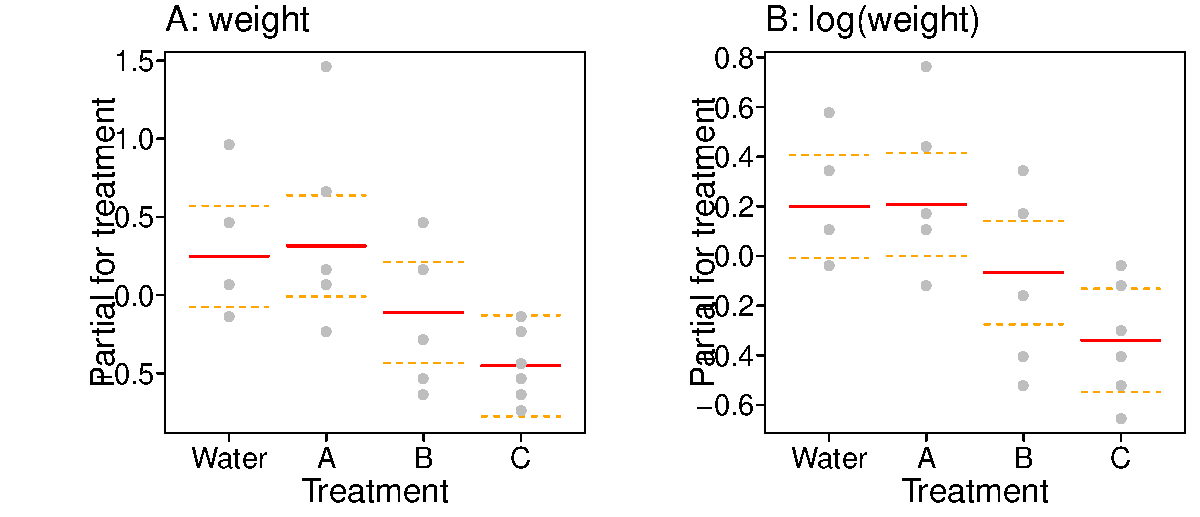
\includegraphics[width=\textwidth]{figs/8-termplot-aovAB-1} }

\end{Schunk}
 \caption{Termplot summary of the one-way analysis of variance result ---
A: for the analysis that uses weights as the outcome variable, and
B: for the analysis that works with \txtt{log(weight)}}
\label{fig:tomatoterm}
\end{figure}

\noindent
Code for Figures \ref{fig:tomatoterm}A and \ref{fig:tomatoterm}B is:
\begin{Schunk}
\begin{Sinput}
## Panel A: Use weight as outcome variable
tomato.aov <- aov(weight ~ trt, data=tomato)
termplot(tomato.aov, xlab="Treatment",
         ylab="Partial for treatment",
         partial.resid=TRUE, se=TRUE, pch=16)
mtext(side=3, line=0.5, "A: weight", adj=0, cex=1.2)
## Panel B: Use log(weight) as outcome variable
logtomato.aov <- aov(log(weight) ~ trt, data=tomato)
termplot(logtomato.aov, xlab="Treatment",
         ylab="Partial for treatment",
         partial.resid=TRUE, se=TRUE, pch=16)
mtext(side=3, line=0.5, "B: log(weight)", adj=0,
      cex=1.2)
\end{Sinput}
\end{Schunk}

Residuals, if required, can be obtained by subtracting the
fitted values in Table \ref{tab:tomatoXmatrixfit} from the observed
values ($y$) in Table \ref{tab:tomatowt}.

Coefficient estimates for the model that uses \txtt{weight} as the
dependent variable, taken from the output summary from R, are:

\begin{Schunk}
\begin{Sinput}
round(coef(summary.lm(tomato.aov)),3)
\end{Sinput}
\begin{Soutput}
            Estimate Std. Error t value Pr(>|t|)
(Intercept)    1.683      0.187   9.019    0.000
trtA           0.067      0.264   0.253    0.803
trtB          -0.358      0.264  -1.358    0.190
trtC          -0.700      0.264  -2.652    0.015
\end{Soutput}
\end{Schunk}

The row labeled \verb!(Intercept)! gives the estimate ($=$ 1.683) for
the baseline, i.e., \verb!Water!.  The remaining coefficients
(differences from the baseline) are:\vspace*{-2pt}
\begin{itemize}
\leftskip-1.3pt
\item[ ]A: weight differs by $0.067$.
\item[ ]B: weight differs by $-0.358$.
\item[ ]C: weight differs by $-0.700$.
\vspace*{-2pt}
\end{itemize}%
Regression calculations have given
us a relatively complicated way to calculate the treatment means!
The methodology shows its power to better effect in more complex
forms of model, where there is no such simple alternative.

Examination of the model matrix can settle any doubt about how to
interpret the coefficient estimates, The first four columns of Table
\ref{tab:tomatoXmatrixfit} comprise the model matrix, given by:
\begin{Schunk}
\begin{Sinput}
model.matrix(tomato.aov)
\end{Sinput}
\end{Schunk}
The multipliers determined by least squares calculations are shown
above each column. Also shown is the fitted
value, which can be calculated either as \txtt{fitted(tomato.aov)} or as
\txtt{predict(tomato.aov)}.
\begin{table}
\tabcolsep9pt
\begin{tabular}{>{\columncolor{light}}l>{\columncolor{light}}l
>{\columncolor{light}}l>{\columncolor{light}}ll@{}}
\rowcolor{white} \color{black}
Water: 1.683 &  A: $+0.067$  &   B:  $-0.358$ &  C:  $-0.700$ & Fitted\\
 & & & & value\\
1&   0&   0&   0&      1.683 \\
1&   0&   0&   0&      1.683 \\
. . . .\\
1&   0&   0&   0&      1.683 \\
1&   1&   0&   0&      1.750 \\
1&   1&   0&   0&      1.750 \\
. . . .\\
1&   1&   0&   0&      1.750 \\
1&   0&   1&   0&      1.325 \\
1&   0&   1&   0&      1.325 \\
. . . .\\
1&   0&   1&   0&      1.325 \\
1&   0&   0&   1&      0.983 \\
1&   0&   0&   1&      0.983 \\
. . . .\\
1&   0&   0&   1&      0.983 \\
\end{tabular}
\caption{The model matrix for the analysis of variance calculation for
  the data in Table~\ref{tab:tomatowt} is shown in gray. A fourth
  column has been added that shows the fitted values.  At the head of
  each column is the multiple, as determined by least squares, that is
  taken in forming the fitted values.
\label{tab:tomatoXmatrixfit}}
\end{table}

\subsection{Factor terms -- different choices of model matrix}

In the language used in the R help pages, different choices of
\textit{contrasts} are available, with each different choice leading
to a different model matrix and to different regression parameters.
The fitted values remain the same, the termplot in Figure {fig:tomatoterm}A
is unchanged, and the analysis of variance table is unchanged.

Where there is just one factor, the constant term can be omitted,
i.e., it is effectively forced to equal zero. The parameters are then
the estimated treatment means. Specify:
\begin{Schunk}
\begin{Sinput}
## Omit constant term from fit;
## force parameters to estimate treatment means
tomatoM.aov <- aov(weight ~ 0 + trt, data=tomato)
\end{Sinput}
\end{Schunk}

The first nine rows of the model matrix are:
\begin{Schunk}
\begin{Sinput}
mmat <- model.matrix(tomatoM.aov)
mmat[1:9, ]
\end{Sinput}
\begin{Soutput}
  trtWater trtA trtB trtC
1        1    0    0    0
2        1    0    0    0
3        1    0    0    0
4        1    0    0    0
5        1    0    0    0
6        1    0    0    0
7        0    1    0    0
8        0    1    0    0
9        0    1    0    0
\end{Soutput}
\begin{Sinput}
## ...   ...    ...    ...
\end{Sinput}
\end{Schunk}
Observe that there is now not an initial column of ones.
This is fine when there is just one factor, but does not generalize to
handle more than one factor and/or factor interaction.

\marginnote[10pt]{Be sure to
choose the contrasts that give the output that will be most helpful
for the problem in hand.  Or, more than one run of the analysis may be
necessary, in order to gain information on all effects that are of
interest.}
The default (\textit{treatment}) choice of \textit{contrasts} uses the
initial factor level as baseline, as we have noted.  Different choices
of the baseline or reference level lead to different versions of the
model matrix.  The other common choice, i.e., \textit{sum} contrasts,
uses the average of treatment effects as the baseline.

\subsection*{The sum contrasts}

Here is the output when the baseline is the average of
the treatment effects, i.e., from using the \textit{sum} contrasts:
\begin{Schunk}
\begin{Sinput}
oldoptions <- options(contrasts=c("contr.sum",
                                  "contr.poly"))
tomatoS.aov <- aov(weight ~ trt, data=tomato)
round(coef(summary.lm(tomatoS.aov)),3)
\end{Sinput}
\begin{Soutput}
            Estimate Std. Error t value Pr(>|t|)
(Intercept)    1.435      0.093  15.381    0.000
trt1           0.248      0.162   1.534    0.141
trt2           0.315      0.162   1.946    0.066
trt3          -0.110      0.162  -0.683    0.502
\end{Soutput}
\begin{Sinput}
options(oldoptions)  # Restore default contrasts
\end{Sinput}
\end{Schunk}
% $\newline
\marginnote[10pt]{The estimates (means) are:
\begin{itemize}
\leftskip-1.5pt
\item[ ] Water: $1.435+0.248 = 1.683$.
\item[ ] A: $1.435+0.315 = 1.750 $.
\item[ ] B: $1.435-0.110 = 1.325$.
\item[ ] C: $1.435-0.452 = 0.983$.
\end{itemize}
}
The baseline, labeled \verb!(Intercept)!, is now
the treatment mean.  This equals 1.435. Remaining coefficients are
differences, for Water and for treatment levels A and B, from this
mean.  The sum of the differences for all three treatments is zero.
Thus the difference for C is (rounding up) \vspace*{-2pt}
\[
-(0.2479+ 0.3146-0.1104) = -0.4521 .\vspace*{-2pt}\]

Yet other choices of contrasts are possible; see
\txtt{help(contrasts)}.

\subsection*{Interaction terms}
The data frame \txtt{cuckoos} has the lengths and breadths of cuckoo
eggs that were laid in the nexts of one of six different bird species.
The following compares a model where the regression line of
breadth against length is the same for all species, with a
model that fits a different line for each different cuckoo species:
\begin{fullwidth}
\begin{Schunk}
\begin{Sinput}
cuckoos.lm <- lm(breadth ~ species + length, data=cuckoos)
cuckoosI.lm <- lm(breadth ~ species + length + species:length, data=cuckoos)
print(anova(cuckoos.lm, cuckoosI.lm), digits=3)
\end{Sinput}
\begin{Soutput}
Analysis of Variance Table

Model 1: breadth ~ species + length
Model 2: breadth ~ species + length + species:length
  Res.Df  RSS Df Sum of Sq    F Pr(>F)
1    113 18.4                         
2    108 17.2  5      1.24 1.56   0.18
\end{Soutput}
\end{Schunk}
\end{fullwidth}

\noindent Here, the model \txtt{cuckoos.lm}, where the regression lines are
parallel (the same slope for each species), appears adequate.
%' The coefficients are:
%' <<cuckoos-ests, echo=2>>=
%' @ %
%' The intercept for the hedge sparrow is 12.403.
%' This has been used as the baseline, with other
%' intercepts given as differences from this.  The slope is
%' 0.189, here assumed the same for all species.

An alternative way to compare the two models is:
\begin{Schunk}
\begin{Sinput}
anova(cuckoos.lm, cuckoosI.lm, test="Cp")
\end{Sinput}
\end{Schunk}
The \txtt{Cp} statistic (smaller is better) compares models on the basis
of an assessment of their predictive power. Note the use of the
argument \txtt{test="cp"}, even though this is not a comparison
that is based on a significance text.

\section{Regression with two explanatory variables}\label{sec:nihills-reg}

\subsection*{Data exploration}

The dataset \txtt{nihills} in the {\em DAAG} package has
record times for Northern Ireland mountain races.  First, get a few
details of the data:
\begin{fullwidth}
\begin{Schunk}
\begin{Sinput}
str(nihills)
\end{Sinput}
\begin{Soutput}
'data.frame':	23 obs. of  4 variables:
 $ dist : num  7.5 4.2 5.9 6.8 5 4.8 4.3 3 2.5 12 ...
 $ climb: int  1740 1110 1210 3300 1200 950 1600 1500 1500 5080 ...
 $ time : num  0.858 0.467 0.703 1.039 0.541 ...
 $ timef: num  1.064 0.623 0.887 1.214 0.637 ...
\end{Soutput}
\end{Schunk}
\end{fullwidth}

The following Figure \ref{fig:nimra-reg} repeats Figure
\ref{fig:nimra} from Chapter \ref{sec:nihills}.
The left panel shows the unlogged data, while the
right panel shows the logged data:
\begin{figure*}
\vspace*{-6pt}
\begin{Schunk}


\centerline{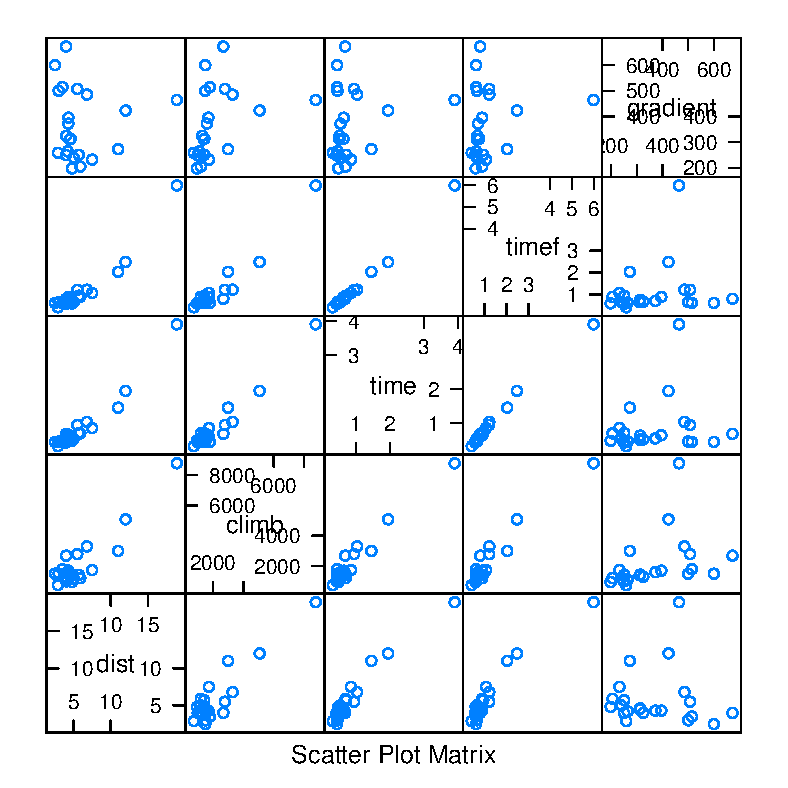
\includegraphics[width=0.48\textwidth]{figs/8-splot2-ni-1} 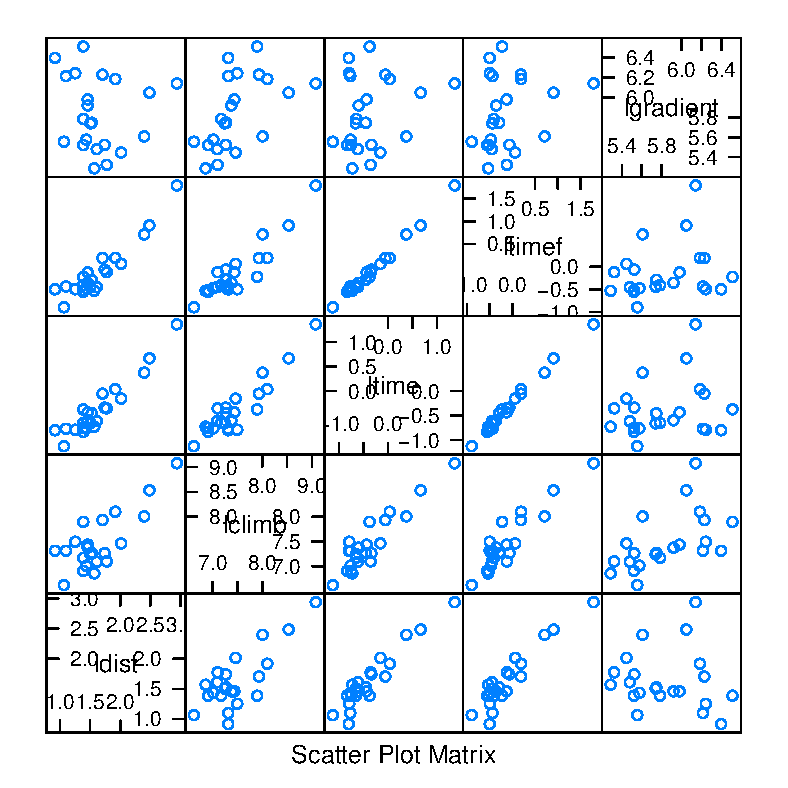
\includegraphics[width=0.48\textwidth]{figs/8-splot2-ni-2} }

\end{Schunk}
\caption{Scatterplot matrices for the Northern Ireland mountain racing
  data. In the right panel, code has been added that shows the
  correlations.
This repeats Figure \ref{fig:nimra} from Chapter \ref{sec:nihills}.
\label{fig:nimra-reg}}
\end{figure*}

The relationships between explanatory variables, and between the
dependent variable and explanatory variables, are closer to linear
when logarithmic scales are used.  Just as importantly, the point with
the largest unlogged values (the same for all variables) will have a
leverage, influencing the fitted regression, that is enormously larger
than that of other points.

The log transformed data are consistent with a form of parsimony that
is well-designed to lead to a simple form of model. We will see that
this also leads to more readily interpretable results.  Also the
distributions for individual variables are more symmetric.

Here again is the code:
\begin{Schunk}
\begin{Sinput}
## Unlogged data
library(lattice)
## Scatterplot matrix; unlogged data
splom(~nihills)
\end{Sinput}
\end{Schunk}

The right panel requires a data frame that has the logged data
\begin{Schunk}
\begin{Sinput}
## Logged data
lognihills <- log(nihills)
names(lognihills) <- paste0("l", names(nihills))
## Scatterplot matrix; log scales
splom(~ lognihills)
\end{Sinput}
\end{Schunk}

\subsection{The regression fit}

The following regression fit uses logarithmic scales for
all variables:

\begin{Schunk}
\begin{Sinput}
lognihills <- log(nihills)
lognam <- paste0("l", names(nihills))
names(lognihills) <- lognam
lognihills.lm <- lm(ltime ~ ldist + lclimb,
                    data=lognihills)
round(coef(lognihills.lm),3)
\end{Sinput}
\begin{Soutput}
(Intercept)       ldist      lclimb 
     -4.961       0.681       0.466 
\end{Soutput}
\end{Schunk}
\marginnote[12pt]{The fitted equation gives predicted times:
\begin{eqnarray*}
 && e^{3.205} \times \mbox{dist}^{0.686} \times
\mbox{climb}^{0.502}\\
 &=& 24.7 e^{3.205} \times \mbox{dist}^{0.686} \times \mbox{climb}^{0.502}
\end{eqnarray*}
}
\noindent
Thus for constant \txtt{climb}, the prediction is that time per mile
will decrease with increasing distance. Shorter races with the same climb
will involve steeper ascents and descents.

A result that is easier to interpret can be obtained by regressing
\txtt{log(time)} on \txtt{log(dist)} and \txtt{log(gradient)},
where \txtt{gradient} is \txtt{dist/climb}.
\begin{Schunk}
\begin{Sinput}
nihills$gradient <- with(nihills, climb/dist)
lognihills <- log(nihills)
lognam <- paste0("l", names(nihills))
names(lognihills) <- lognam
lognigrad.lm <- lm(ltime ~ ldist + lgradient,
                   data=lognihills)
round(coef(lognigrad.lm),3)
\end{Sinput}
\begin{Soutput}
(Intercept)       ldist   lgradient 
     -4.961       1.147       0.466 
\end{Soutput}
\end{Schunk}
Thus, with \txtt{gradient} held constant, the prediction is that \txtt{time}
will increase at the rate of $\mbox{dist}^{1.147}$.  This makes good intuitive
sense.

\begin{figure}
\begin{Schunk}


\centerline{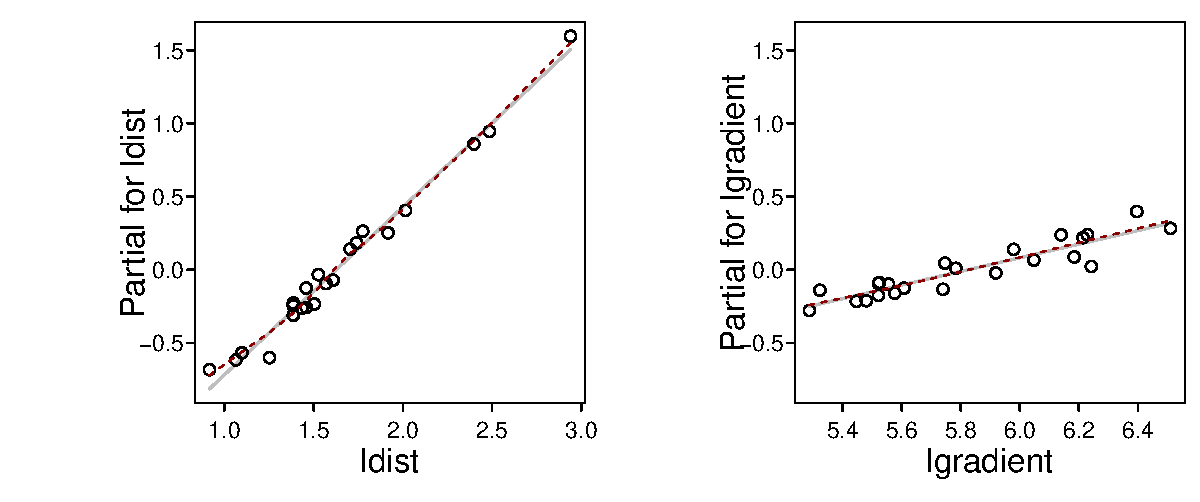
\includegraphics[width=\textwidth]{figs/8-tplot-ni-1} }

\end{Schunk}
\caption{The vertical scales in both ``term plot''  panel
  show $\log(\rm{time})$, centered to a mean of zero. The partial residuals
  in the left panel are for $\txtt{ldist}$, while those in the right
  panel are for $\txtt{lgradient}$, i.e.,
  \txtt{log(climb/dist)}. Smooth curves (dashes) have been passed
  through the points.\label{fig:lnihills-lin}}
\vspace*{-5pt}
\end{figure}

We pause to look more closely at the model that has been fitted.  Does
\txtt{log(time)} really depend linearly on the terms \txtt{ldist} and
\txtt{log(lclimb)}?  The function \txtt{termplot()} gives a good
graphical indication (Figure \ref{fig:lnihills-lin}).
\begin{Schunk}
\begin{Sinput}
## Plot the terms in the model
termplot(lognigrad.lm, col.term="gray", partial=TRUE,
         col.res="black", smooth=panel.smooth)
\end{Sinput}
\end{Schunk}

The vertical scales show changes in \txtt{ltime}, about the mean of
\txtt{ltime}.  The lines show the estimated effect of each explanatory
variable when the other variable is held at its mean value.  The
lines, which are the contributions of the individual linear terms
(``effects'') in this model, are shown in gray so that they do not
obtrude unduly. The dashed curves, which are smooth curves that are
passed through the residuals, are the primary features of interest.

Notice that, in the plot for \txtt{ldist}, the smooth dashed line does
not quite track the fitted line; there is a small but noticeable
indication of curvature that can be very adequately modeled with a
quadratic curve.  Note also that until we have modeled effectively the
clear trend that seems evident in this plot, there is not much
point in worrying about possible outliers.

\section{Variable Selection -- Stepwise and Other}\label{ss:varsel}

Common variable selection methods include various versions of forward
and backward selection, and exhaustive (best subset) selection.  These
or other variable selection methods invalidate standard model
assumptions, which assume a single known model.

There are (at least) three inter-related issues for the use of results
from a variable selection process:
\marginnote[-12pt]{The points made here can have highly damaging
  implications for analyses where it is important to obtain
  interpretable regression coefficients.  In such analyses, changes to
  the initial model should be limited to simplifications that do not
  modify the model in any substantial manner.  Following the selection
  process, check coefficients against those from the full model.  Any
  large changes should ring a warning bell.

  The implications for prediction are, relatively, much more
  manageable. The key requirement is to use independent data to show
  that any selective process has genuinely improved model
  performance.}
\begin{enumerate}
\item[(i)] Use of standard theoretically based model fitting procedures,
  applied to the model that results from the model selection process,
  will lead to a spuriously small error variance, and to a spuriously
  large model $F$-statistic.  Coefficient estimates will be inflated,
  have spuriously small standard errors, and spuriously large
  $t$-statistics.  (Or to put the point another way, it is inappropriate
  to refer such statistics to a standard $t$-distribution.)
\item[(ii)] Commonly used stepwise and other model selection processes
  are likely to over-fit, i.e., the model will not be optimal for
  prediction on test data that are distinct from the data used to
  train the model.  The selected model may in some instances be
  inferior, judged by this standard, to a model that uses all candidate
  explanatory variables. (There are alternative ways to use all variables.
  Should low order interactions be included?  Should some variables be
  transformed?)
\item[(iii)] Coefficients may change, even to changing in sign, depending
  on what else is included in the model. With a different total set of
  coefficients, one has a different model, and the coefficients that
  are common across the two models may be accordingly different.
  (They will be exactly the same only in the unusual case where
  ``variables'' are uncorrelated.)  There is a risk that variable
  selection will remove variables on whose values (individually, or in
  total effect) other coefficient estimates should be conditioned.
  This adds uncertainty beyond what arises from sampling variation.
  \label{item:coef}
\end{enumerate}

Note that these points apply to pretty much any type of regression
modelling, including generalized linear models and classification
(discriminant) models.

Where observations are independent, items (i) and (ii) can be
addressed, for any given selection process, by splitting the data into
training, validation and test sets.  Training data select the model,
with the validation data used to tune the selection process.
Model performance is then checked against the test data.

Somewhat casual approaches to the use of backward (or other) stepwise
selection may be a holdover from hand calculator days, or from times
when computers grunted somewhat to handle even modest sized
calculations.  This may be one of the murky dark alleys of statistical
practice, where magic incantations and hope too often prevail over
hard evidence.

Appropriate forms of variable selection process can however be
effective in cases where a few only of the coefficients have
predictive power, and the relevant $t$-statistics are large --
too large to be substantially inflated by selection effects.

\subsection{Use of simulation to check out selection effects:}
The function \txtt{bestsetNoise()} ({\em DAAG}) can be used to
experiment with the behaviour of various variable selection techniques
with data that is purely noise.  For example, try:\sidenote{See also
Section 6.5, pp.~197-198, in:
  Maindonald, JH and Braun, WJ, 2010. \textit{Data Analysis
    and Graphics Using R -- An Example-Based Approach\/}, 3$^{rd}$
  edition. Cambridge University Press.}
\begin{Schunk}
\begin{Sinput}
bestsetNoise(m=100, n=40, nvmax=3)
bestsetNoise(m=100, n=40, method="backward",
             nvmax=3)
\end{Sinput}
\end{Schunk}
The analyses will typically yield a model that appears to
have highly (but spuriously) statistically significant explanatory power,
with one or more coefficients that appear (again spuriously)
significant at a level of around $p$=0.01 or less.

\paragraph{The extent of selection effects -- a detailed simulation:}
As above, datasets of random normal data were created, always with 100
observations and with the number of variables varying between 3 and
50.  For three variables, there was no selection, while in other cases
the ``best'' three variables were selected, by exhaustive search.

\begin{marginfigure}
\begin{Schunk}


\centerline{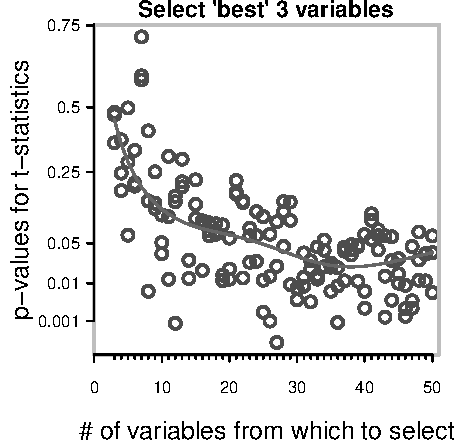
\includegraphics[width=\textwidth]{figs/8-bsnVary-1} }

\end{Schunk}
\caption{$p$-values, versus number of variables available for selection,
  when the ``best'' 3 variables were selected by exhaustive search.
  The fitted line estimates the median $p$-value.\label{fig:exhaust}}
\end{marginfigure}
\noindent

Figure \ref{fig:exhaust} plots the p-values for the 3 variables that
were selected against the total number of variables. The fitted line
estimates the median $p$-value.
Code is:
\begin{Schunk}
\begin{Sinput}
library(DAAG)
library(quantreg)
library(splines)
set.seed(37)   # Use to reproduce graph shown
bsnVaryNvar(m=100, nvar=3:50, nvmax=3, fg="gray")
\end{Sinput}
\end{Schunk}

When all 3 variables are taken, the $p$-values are expected to average
0.5.  Notice that, for selection of the best 3 variables out of 10,
the median $p$-value has reduced to about 0.1.

\paragraph{Examples from the literature}

The paper cited in the sidenote\sidenote{Ambroise, C and McLachlan,
  GJ, 2001. Selection bias in gene extraction on the basis of
  microarray gene-expression data.  \textit{Proceedings of the
    National Academy of Sciences USA}, \textbf{99}: 6562-6566.} gives
several examples of published spurious results, all for the use of
discriminant methods with microarray data.  The same effects can arise
from model tuning.

\subsection{Variable and model selection -- strategies}

Several alternative mechanisms are available that can yield reasonable
standard errors and other accuracy measures. These include:
\begin{itemizz}
\item[a)] Fit the model to test data that have played no part in
the model selection and tuning process;
\item[b)] use cross-validation.  The model selection and fitting
process must be repeated at each cross-validation fold;
\item[c)] repeat the whole analysis, selection and all, with repeated
 bootstrap samples, using variation between the different sample
results to assess the accuracy of one or other statistic;
\item[d)] simulate, including all selection and tuning steps, from the
  fitted model.
\end{itemizz}
For b) and c), there will be somewhat different selections for each
different cross-validation fold or bootstrap sample.  This is itself
instructive.

One possibility,\marginnote{If however the coefficients are not themselves very meaningful, what is the point?}
following stepwise or other selection, is that the
$p$-values of one or more coefficients may be so small that they are
very unlikely to be an artefact of the selection process.  In general,
a simulation will be required, in order to be sure.

\subsection*{Model selection more generally:}

More generally, \marginnote{Use of test data that are separate
from data used to develop the model deals with this issue.}
the model may be chosen from a wide class of models.
Again, model selection biases standard errors to be smaller than
indicated by the theory, and coefficients and $t$-statistics larger.
The resulting anti-conservative estimates of standard errors and
other statistics should be regarded
sceptically. 

A further issue, which use of separate test data does not
  address, is that none of the models on offer is likely to be
  strictly correct. Mis-specification of the fixed effects will bias
  model estimates, at the same time inflating the error variance or
  variances.  Thus it will to an extent work in the opposite direction
  to selection effects.

\section{1970 cost for US electricity producers}\label{ss:elec}

There is a wide range of possible choices of model terms.
Figure \ref{fig:elec-spm} shows the scatterplot matrices of the
variables. Code is:
\begin{Schunk}
\begin{Sinput}
library(car)
library(Ecdat)
data(Electricity)
spm(Electricity, smooth=TRUE, regLine=FALSE,
    col=adjustcolor(rep("black",3), alpha.f=0.3))
\end{Sinput}
\end{Schunk}

\begin{figure*}[h]
\vspace*{-18pt}
\parbox[c]{0.7\textwidth}{
\begin{Schunk}


\centerline{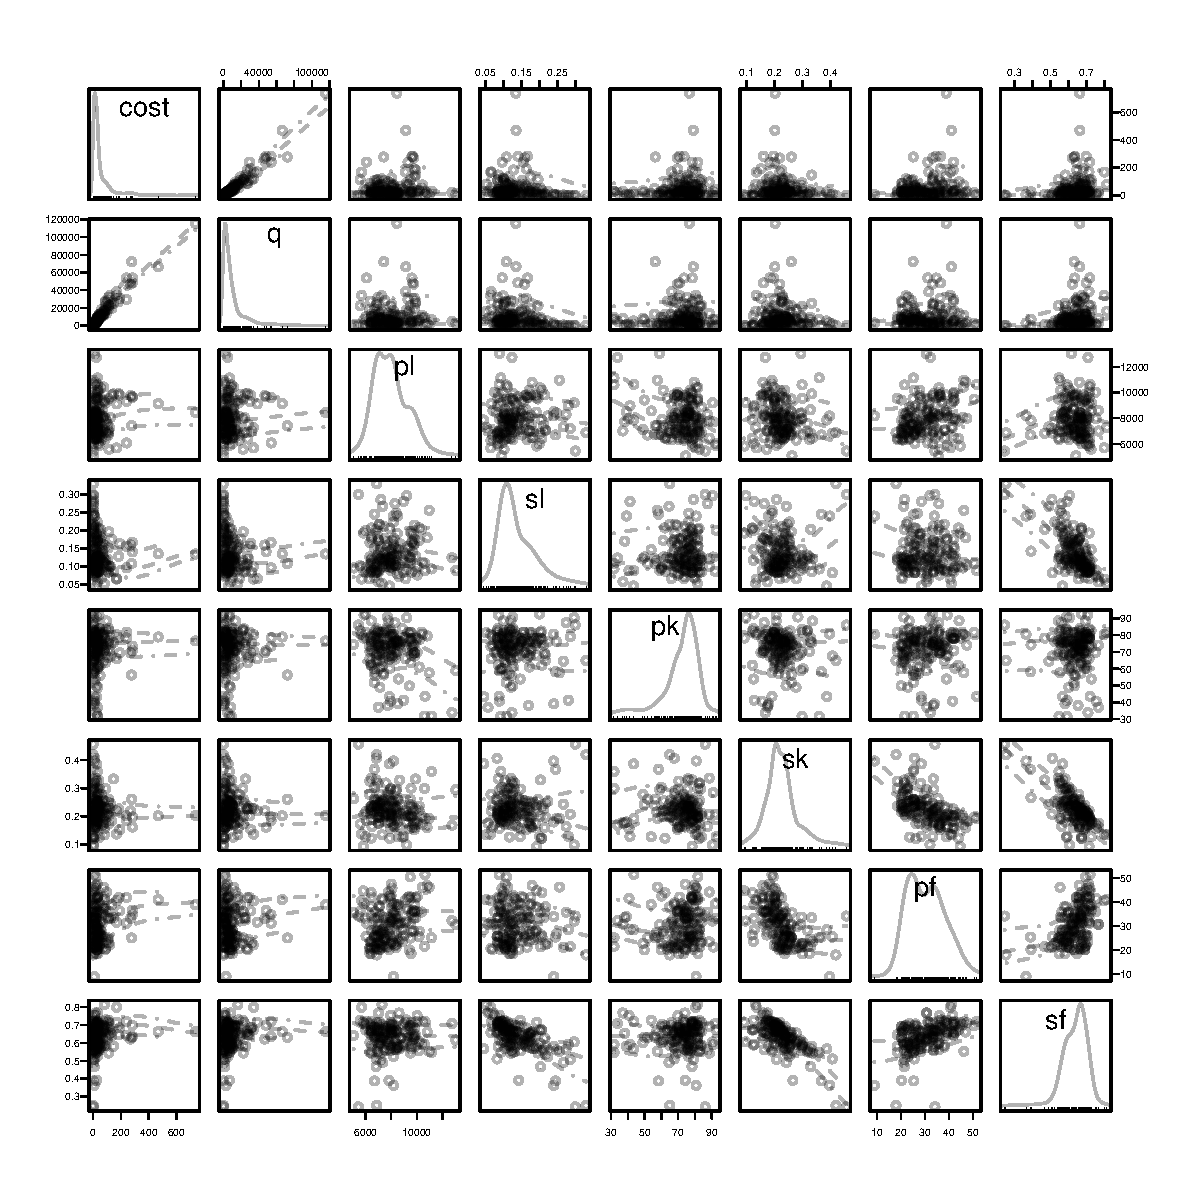
\includegraphics[width=0.775\textwidth]{figs/8-Elec-spm-1} }

\end{Schunk}
}
\hspace*{0.05\textwidth}
\parbox[c]{0.23\linewidth}{
\small
\begin{list}{}{\leftmargin=2em \setlength{\itemsep}{5pt} \setlength{\parsep}{1pt}}
\setlength{\labelwidth}{3em}
\item[\texttt{cost:}]
 total cost
\item[\texttt{q:}]
 total output
\item[\texttt{pl:}]
 wage rate
\item[\texttt{sl:}]
 cost share, labor
\item[\texttt{pk:}]
 capital price index
\item[\texttt{sk:}]
 cost share,
 capital
\item[\texttt{pf:}]
 fuel price
\item[\texttt{sf:}]
 cost share, fuel
\end{list}
}
\vspace*{-9pt}

\caption{Scatterplot matrix, for the variables in the data set
  \texttt{Electricity}, in the {\em Ecdat} package. Density
  plots are shown in the diagonal.\label{fig:elec-spm}}
\end{figure*}

\subsection{Model fitting strategy}

The analysis will start by checking for clearly desirable
transformations to variables.  Then, for obtaining a model whose
whose parameters are as far as possible interpretable, a strategy
is:
 \begin{itemize}
 \item[(i)] Start with a model that includes all plausible main effects
   (variables and factors).  Ensure that the model is parameterised in
   a way that makes parameters of interest as far as possible
   interpretable (e.g., in Subsection \ref{sec:nihills} above, work
   with \texttt{distance} and \texttt{gradient}, not \texttt{distance}
   and \texttt{climb})
 \item[(ii)]
 \marginnote{Removal of terms with $p > 0.15$ or $p > 0.2$
     rather than $p$ > 0.05 greatly reduces the risk that estimates of
     other parameters, and their standard errors, will change in ways
     that affect the interpretation of model results.}[21pt]
   Model simplification may be acceptable, if it does not
   change the parameters of interest to an extent that affects
   interpretation. The common $p$ > 0.05 is too
   severe; try instead
   $p$ = 0.15 (remove terms with $p > 0.15$) or $p$ = 0.20.
 \item[(iii)] Variables and/or factors that have no detectable main
   effect are in general unlikely to show up in interactions.
   Limiting attention to the main effects that were identified in (ii)
   above, we then compare a model which has only main effects with a
   model that inludes all 2-way interactions. Then, using $p$ $\simeq$
   0.15 or $p$ $\simeq$ 0.2 as the cutoff, remove interaction terms
   that seem unimportant, and check that there are no changes of
   consequence in terms that remain.
 \item[(iv)] In principle, the process may be repeated for order 3
   interactions.
\item[(v)] Use the function \txtt{add1()} to check for individual
highly significant terms that should be included.  For this purpose,
we might set $p=0.01$ or perhaps $p=0.001$.
\end{itemize}
The strategy is to be cautious (hence the cutoff of $p=0.2$) in
removing terms, whether main effects or first order interactions.
In a final check whether there is a case for adding in terms that
had been omitted, we include a term only if it is highly statistically
significant.  This limits the scope for selection effects.

\subsection*{Distributions of variables}

The distributions of \texttt{cost} and \texttt{q} are highly skew.
The relationship between these two variables is also very close to
linear.  We might try taking logarithms of both these variables.

Figure \ref{fig:elec-dens} examines the scatterplot matrix for the
logarithms of the variables \txtt{cost} and \txtt{q}.
\noindent
Code is:
\begin{marginfigure}[-3.5cm]
\begin{Schunk}


\centerline{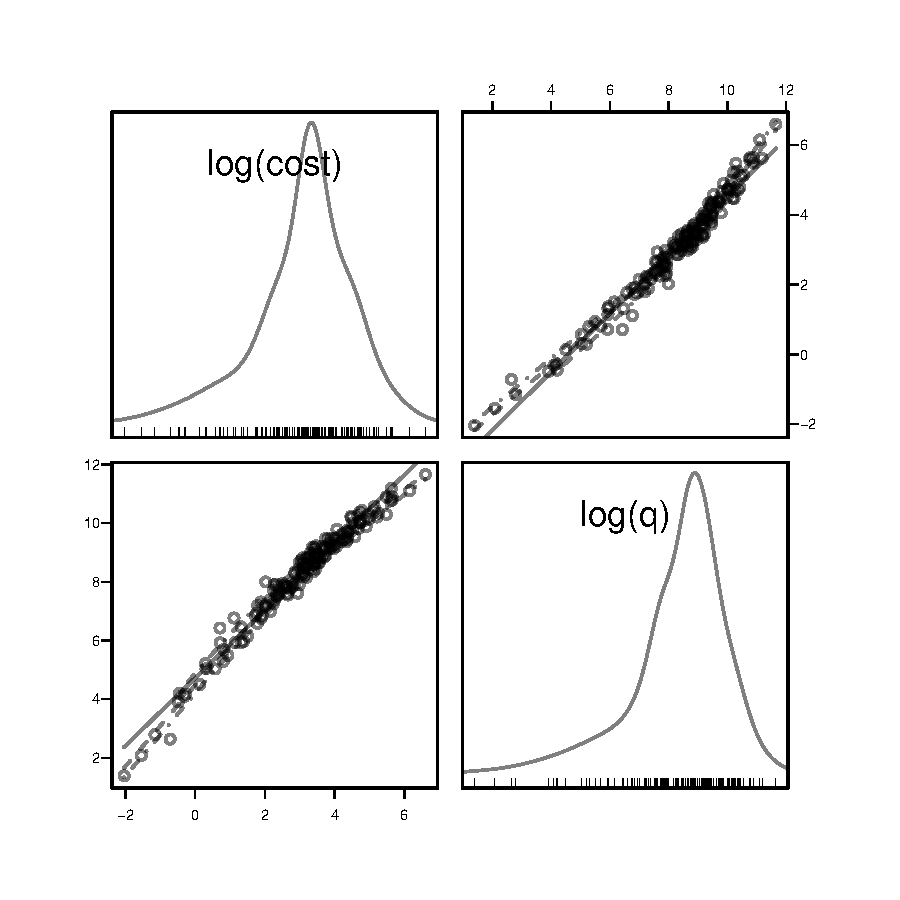
\includegraphics[width=\textwidth]{figs/8-spm-cost-q-1} }

\end{Schunk}
  \caption{Scatterplot matrix for the logarithms of the variables
    \txtt{cost} and \txtt{q}. Density plots are shown in the
    diagonal.\label{fig:elec-dens}}
\end{marginfigure}
\begin{Schunk}
\begin{Sinput}
varlabs <- c("log(cost)", "log(q)")
spm(log(Electricity[,1:2]), var.labels=varlabs,
    smooth=TRUE, regLine=FALSE,
    col=adjustcolor(rep("black",3), alpha.f=0.5))
\end{Sinput}
\end{Schunk}
We start with a model that has main effects only:
\begin{Schunk}
\begin{Sinput}
elec.lm <- lm(log(cost) ~ log(q)+pl+sl+pk+sk+pf+sf,
              data=Electricity)
\end{Sinput}
\end{Schunk}

Now examine the termplot (Figure \ref{fig:elec-log-tplot}):
\setkeys{Gin}{width=0.95\textwidth}
\begin{figure}[h]
\begin{Schunk}


\centerline{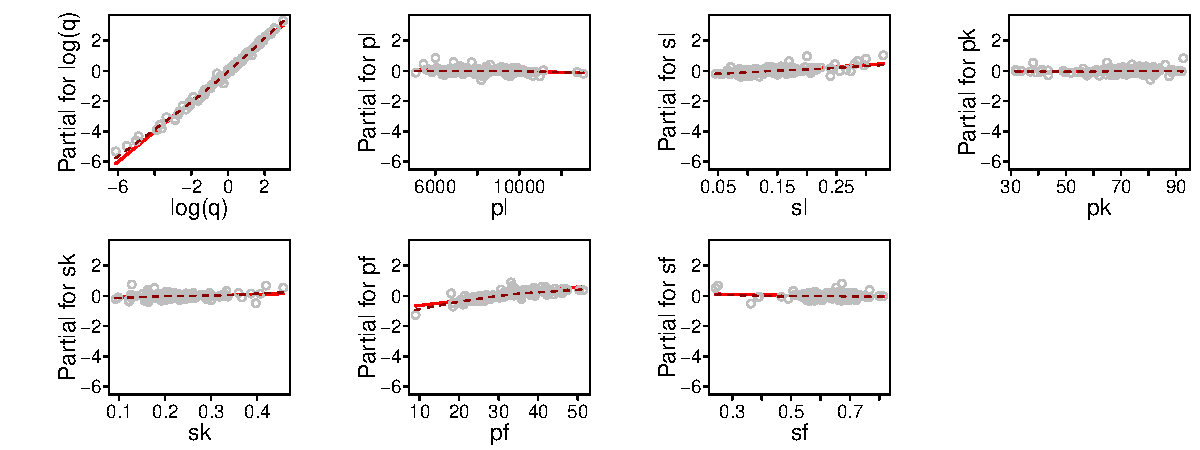
\includegraphics[width=\textwidth]{figs/8-elec-me-tplot-1} }

\end{Schunk}
\caption{Termplot summary for the model that has been fitted to the
  \texttt{Electricity} dataset.\label{fig:elec-log-tplot}}
\end{figure}
\noindent Code is:
\begin{Schunk}
\begin{Sinput}
termplot(elec.lm, partial=T, smooth=panel.smooth,
         transform.x=TRUE)
\end{Sinput}
\end{Schunk}
Notice that in the partial plot for \txtt{q}, the dashed curve that is
fitted to the residuals closely tracks the fitted effect (linear on a
scale of \txtt{log(q)}.  This confirms the use of \txtt{log(q)},
rather than \txtt{q}, as explanatory variable.

Now examine the model output:
\begin{Schunk}
\begin{Sinput}
round(coef(summary(elec.lm)),5)
\end{Sinput}
\begin{Soutput}
            Estimate Std. Error t value Pr(>|t|)
(Intercept) -5.41328    0.70720 -7.6545  0.00000
log(q)       0.89250    0.00994 89.8326  0.00000
pl          -0.00002    0.00001 -1.9341  0.05499
sl           2.48020    0.74898  3.3114  0.00116
pk           0.00083    0.00127  0.6562  0.51272
sk           0.62272    0.70837  0.8791  0.38076
pf           0.03042    0.00228 13.3338  0.00000
sf          -0.30965    0.69091 -0.4482  0.65467
\end{Soutput}
\end{Schunk}

The $p$-values suggest that \texttt{pk}, \texttt{sk}, and \texttt{sf}
can be dropped from the model. Omission of these terms makes only
minor differences to the coefficients of terms that remain.
\begin{Schunk}
\begin{Sinput}
elec2.lm <- lm(log(cost) ~ log(q)+pl+sl+pf,
               data=Electricity)
round(coef(summary(elec2.lm)),5)
\end{Sinput}
\begin{Soutput}
            Estimate Std. Error t value Pr(>|t|)
(Intercept) -5.28641    0.13701 -38.585  0.00000
log(q)       0.88901    0.00986  90.167  0.00000
pl          -0.00002    0.00001  -2.072  0.03994
sl           2.69722    0.32464   8.308  0.00000
pf           0.02659    0.00191  13.934  0.00000
\end{Soutput}
\end{Schunk}

Now check whether interaction terms should be included:
\begin{Schunk}
\begin{Sinput}
elec2x.lm <- lm(log(cost) ~ (log(q)+pl+sl+pf)^2,
                data=Electricity)
anova(elec2.lm, elec2x.lm)
\end{Sinput}
\begin{Soutput}
Analysis of Variance Table

Model 1: log(cost) ~ log(q) + pl + sl + pf
Model 2: log(cost) ~ (log(q) + pl + sl + pf)^2
  Res.Df  RSS Df Sum of Sq    F  Pr(>F)
1    153 5.00                          
2    147 2.81  6      2.19 19.1 2.3e-16
\end{Soutput}
\end{Schunk}
The case for including first order interactions seems strong. The
coefficients and SEs are:
\begin{Schunk}
\begin{Sinput}
round(coef(summary(elec2x.lm)),5)
\end{Sinput}
\begin{Soutput}
            Estimate Std. Error t value Pr(>|t|)
(Intercept) -3.63931    0.67803 -5.3675  0.00000
log(q)       0.71481    0.05455 13.1039  0.00000
pl          -0.00031    0.00007 -4.2508  0.00004
sl           6.06389    1.64592  3.6842  0.00032
pf           0.01592    0.01499  1.0623  0.28985
log(q):pl    0.00003    0.00001  6.2902  0.00000
log(q):sl   -0.67829    0.10229 -6.6308  0.00000
log(q):pf    0.00080    0.00113  0.7133  0.47680
pl:sl        0.00007    0.00018  0.4144  0.67916
pl:pf        0.00000    0.00000  0.1421  0.88722
sl:pf        0.01680    0.03092  0.5432  0.58780
\end{Soutput}
\end{Schunk}
This suggests omitting the terms \txtt{pf}, and all interactions
except \txtt{log(q):pl} and \txtt{log(q):sl}.  We check that omission
of these terms makes little difference to the terms that remain:
\begin{Schunk}
\begin{Sinput}
elec2xx.lm <- lm(log(cost) ~ log(q)+pl+sl+pf+
                 log(q):pl+log(q):sl,
                 data=Electricity)
round(coef(summary(elec2xx.lm)),5)
\end{Sinput}
\begin{Soutput}
            Estimate Std. Error t value Pr(>|t|)
(Intercept) -4.12003    0.33312 -12.368        0
log(q)       0.74902    0.03852  19.445        0
pl          -0.00029    0.00004  -7.755        0
sl           7.29642    0.70758  10.312        0
pf           0.02611    0.00145  18.017        0
log(q):pl    0.00003    0.00000   7.657        0
log(q):sl   -0.68969    0.09435  -7.310        0
\end{Soutput}
\end{Schunk}

Now check whether there is a strong case for adding in any further
individual terms:
\begin{fullwidth}
\begin{Schunk}
\begin{Sinput}
add1(elec2xx.lm, scope=~(log(q)+pl+sl+pk+sk+pf+sf)^2, test="F")
\end{Sinput}
\begin{Soutput}
Single term additions

Model:
log(cost) ~ log(q) + pl + sl + pf + log(q):pl + log(q):sl
          Df Sum of Sq  RSS  AIC F value Pr(>F)
<none>                 2.83 -622               
pk         1    0.0041 2.82 -620    0.22   0.64
sk         1    0.0329 2.79 -621    1.76   0.19
sf         1    0.0294 2.80 -621    1.58   0.21
log(q):pf  1    0.0040 2.82 -620    0.21   0.64
pl:sl      1    0.0060 2.82 -620    0.32   0.57
pl:pf      1    0.0004 2.83 -620    0.02   0.88
sl:pf      1    0.0016 2.83 -620    0.09   0.77
\end{Soutput}
\end{Schunk}
\end{fullwidth}

\section{An introduction to logistic regression}\label{sec:logistic}
\marginnote[11pt]{The dataset \margtt{bronchit} may alternatively be found
  in the {\em SMIR} package.}
The data that will be used for illustration are from the data frame
\txtt{bronchit} in the {\em DAAGviz} package.  The following loads
packages that will be needed:

\begin{Schunk}
\begin{Sinput}
library(DAAGviz, quietly=TRUE)
library(KernSmooth, quietly=TRUE)
\end{Sinput}
\end{Schunk}

Figure \ref{fig:cig-poll} shows two plots -- one of \texttt{poll}
(pollution level) against \texttt{cig} (number of cigarettes per day),
and the other of \texttt{poll} against \texttt{log(poll)}.  In each
case, points are identified as with or without bronchitis.

\begin{figure*}
\begin{Schunk}


\centerline{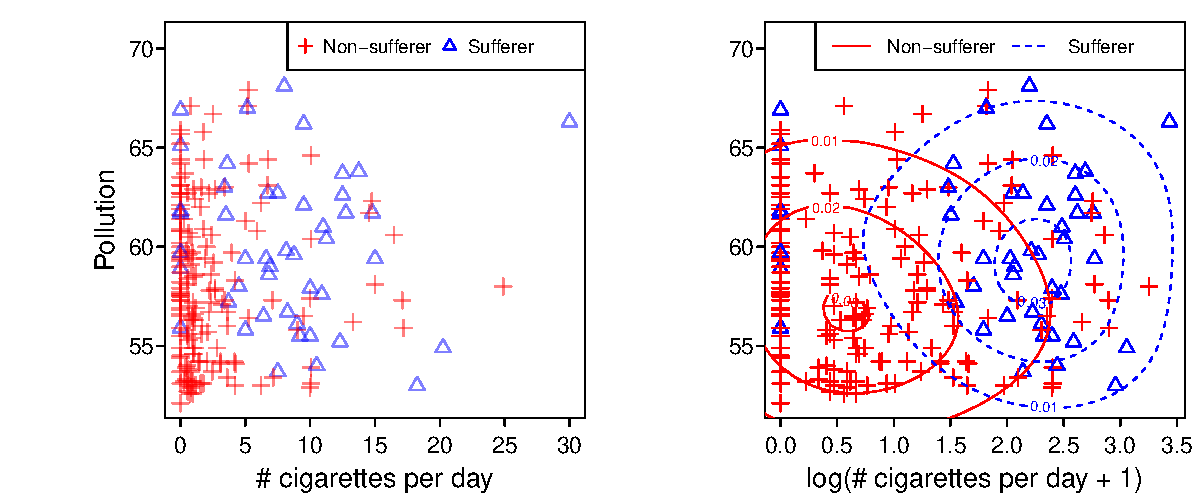
\includegraphics[width=0.95\textwidth]{figs/8-bronchitAB-1} }

\end{Schunk}
\caption{Panel A plots \txtt{poll} (pollution level) against
  \txtt{cig} (number of cigarettes per day).  In panel B, the
  $x$-scale shows the logarithm of the number of cigarettes per
  day.\label{fig:cig-poll}}
\vspace*{12pt}
\end{figure*}

\begin{Schunk}
\begin{Sinput}
## Panel A
colr <- adjustcolor(c("red","blue"), alpha=0.5)
plot(poll ~ cig,
     xlab="# cigarettes per day", ylab="Pollution",
     col=colr[r+1], pch=(3:2)[r+1], data=bronchit,
     ylim=ylim)
legend(x="topright",
       legend=c("Non-sufferer","Sufferer"),
       ncol=2, pch=c(3,2), col=c(2,4), cex=0.8)
\end{Sinput}
\end{Schunk}

%$

\begin{fullwidth}
\begin{Schunk}
\begin{Sinput}
## Panel B
plot(poll ~ log(cig+1), col=c(2,4)[r+1], pch=(3:2)[r+1],
     xlab="log(# cigarettes per day + 1)", ylab="", data=bronchit, ylim=ylim)
xy1 <- with(subset(bronchit, r==0), cbind(x=log(cig+1), y=poll))
xy2 <- with(subset(bronchit, r==1), cbind(x=log(cig+1), y=poll))
est1 <- bkde2D(xy1, bandwidth=c(0.7, 3))
est2 <- bkde2D(xy2, bandwidth=c(0.7, 3))
lev <- pretty(c(est1$fhat, est2$fhat),4)
contour(est1$x1, est1$x2, est1$fhat, levels=lev, add=TRUE, col=2)
contour(est2$x1, est2$x2, est2$fhat, levels=lev, add=TRUE, col=4, lty=2)
legend(x="topright", legend=c("Non-sufferer","Sufferer"), ncol=2, lty=1:2,
\end{Sinput}
\end{Schunk}
\end{fullwidth}

The logarithmic transformation spreads the points out in the
$x$-direction, in a manner that is much more helpful for prediction
than the untransformed values in panel A.  The contours for
non-sufferer and sufferer in panel B have a similar shape.  The
separation between non-sufferer and sufferer is stronger in the
$x$-direction than in the $y$-direction.  As one indication of this,
the contours at a density of 0.02 overlap slightly in the $x$-direction,
but strongly in the $y$-direction.

\subsection*{Logistic regression calculations}

Figure \ref{fig:cig-poll} made it clear
that the distribution of number of cigarettes had a strong positive
skew.  Thus, we might fit the model:
\begin{fullwidth}
\begin{Schunk}
\begin{Sinput}
cig2.glm <- glm(r ~ log(cig+1) + poll, family=binomial, data=bronchit)
summary(cig2.glm)
\end{Sinput}
\begin{Soutput}

Call:
glm(formula = r ~ log(cig + 1) + poll, family = binomial, data = bronchit)

Deviance Residuals: 
   Min      1Q  Median      3Q     Max  
-1.611  -0.586  -0.362  -0.239   2.653  

Coefficients:
             Estimate Std. Error z value Pr(>|z|)
(Intercept)  -10.7877     2.9885   -3.61  0.00031
log(cig + 1)   1.2882     0.2208    5.83  5.4e-09
poll           0.1306     0.0494    2.64  0.00817

(Dispersion parameter for binomial family taken to be 1)

    Null deviance: 221.78  on 211  degrees of freedom
Residual deviance: 168.76  on 209  degrees of freedom
AIC: 174.8

Number of Fisher Scoring iterations: 5
\end{Soutput}
\end{Schunk}
\end{fullwidth}

\begin{figure}[h]
\begin{Schunk}


\centerline{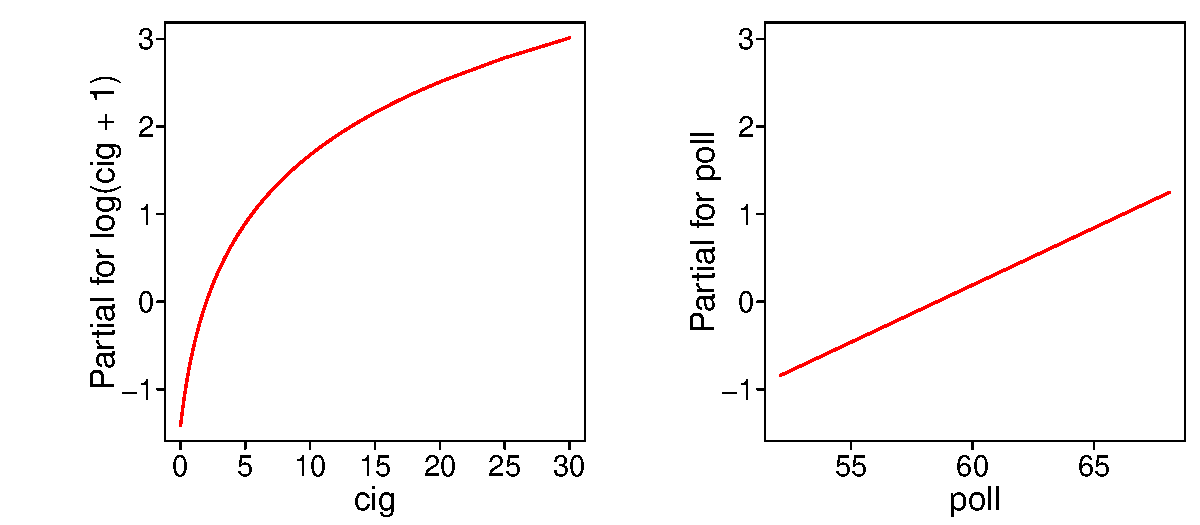
\includegraphics[width=\textwidth]{figs/8-cig2-tplot-1} }

\end{Schunk}
\caption{The panels show the contributions that the respective terms
  make to the fitted values (logit of probability of bronchitis), when
  the other term is held constant.\label{fig:xy-cig}}
\end{figure}

Termplots (Figure \ref{fig:xy-cig}) provide a useful summary of the
contributions of the covariates.  For binary (0/1) data such as here,
including the data values provides no visually useful information.
Code is:
\begin{Schunk}
\begin{Sinput}
termplot(cig2.glm)
\end{Sinput}
\end{Schunk}

\section{Regression with Fitted Smooth Curves}

Load the {\em DAAG} package:


\subsection*{Commentary  on Smoothing Methods}

Two types of methods will be described -- those where the user
controls the choice of smoothing parameter, and statistical learning
type methods where the amount of smoothing is chosen automatically:
\begin{itemize}
\item The first class of methods rely on the user to make a suitable
  choice of a parameter that controls the smoothness.  The default
choice is often a good first approximation.  Note here:
\begin{itemize}
\item Smoothing using a ``locally weighted regression
smoother''.\marginnote{Smoothness
is controlled by the width of the smoothing window. The default is
  \txtt{f=2/3} for \txtt{lowess()}, or \txtt{span=0.75} for
  \txtt{loess()}. For other functions that rely on this methodology,
check the relevant help page.}
Functions that use this approach include \txtt{lowess()}, \txtt{loess()},
\txtt{loess.smooth()}, and \txtt{scatter.smooth()}.
\item Use of a regression spline basis in a linear model.  Here the smoothness
is usually controlled by the choice of number of spline basis terms.
\end{itemize}
\item A second class of methods use a ``statistical learning''
  approach in which the amount of smoothing is chosen automatically.
  The approach of the \textit{mgcv} package extends and adapts the
  regression spline approach.\sidenote{Strong assumptions are
    required, notably that observations are independent.  Normality
    assumptions are, often, less critical.}  The methodology
  generalizes to handle more general types of outcome variables,
  including proportions and counts.  These extensions will not be
  further discussed here.
\end{itemize}

\subsection{Locally weighted scatterplot smoothers}

Locally weighted scatterplot smoothers pass a window across
the data, centering the window in turn at each of a number points that
are equally spaced through the data. The smooth at an $x$-value where
the window has been centred is the predicted value from a line (or
sometimes a quadratic or other curve) that is fitted to values that
lie within the window. A weighted fit is used, so that neighbouring
points get greater weight than points out towards the edge of the
window.

Figure \ref{fig:fruitohms} shows a smooth that has been fitted using
the \txtt{lowess} (locally weighted scatterplot smoothing)
methodology.  The default choice of with of smoothing window (a fraction
$f = \frac{2}{3}$ of the total range of $x$) gives a result that,
for these data, looks about right. The curve does however trend
slightly upwards at the upper end of its range.  A monotonic
response might seem more appropriate.

\begin{marginfigure}
\begin{Schunk}


\centerline{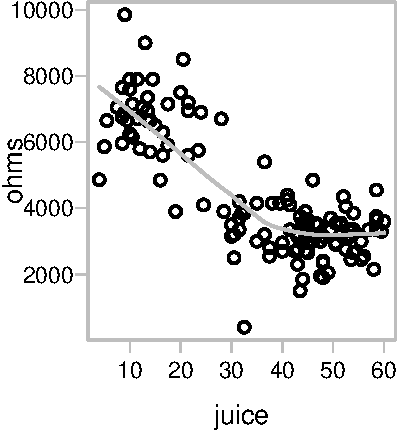
\includegraphics[width=0.98\textwidth]{figs/8-smooth-ohms-1} }

\end{Schunk}
  \caption{Resistance in ohms is plotted against apparent juice
    content.  A smooth curve (in gray) has been added, using the
    \txtt{lowess} smoother.  The width of the smoothing window was the
    default fraction $f = \frac{2}{3}$ of the range of values of the
    $x$-variable.}\label{fig:fruitohms}
\end{marginfigure}

The code used to plot the graph is:
\begin{Schunk}
\begin{Sinput}
## Plot points
plot(ohms ~ juice, data=fruitohms, fg="gray")
## Add smooth curve, using default
## smoothing window
with(fruitohms,
     lines(lowess(ohms ~ juice), col="gray", lwd=2))
\end{Sinput}
\end{Schunk}

A more sophisticated approach uses the \txtt{gam()} function
in the {\em mgcv} package.  This allows automatic determination of the
amount of smoothing, providing the assumption of independent residuals
from the curve is reasonable.  We now demonstrate the use of a GAM
model for a two-dimensional smooth.

\subsection{Contours from 2-dimensional Smooths}
Data are the amplitudes of responses to a visual stimulus, for each of
20 individuals, at different regions of the left eye.  We use the
function \txtt{gam()} to create smooth
surfaces, for males and females separately. Figure \ref{fig:visAmp}
then uses the function \txtt{vis.gam()} to plot heatmaps that show the
contours:
\begin{fullwidth}
\begin{figure*}
\begin{Schunk}


\centerline{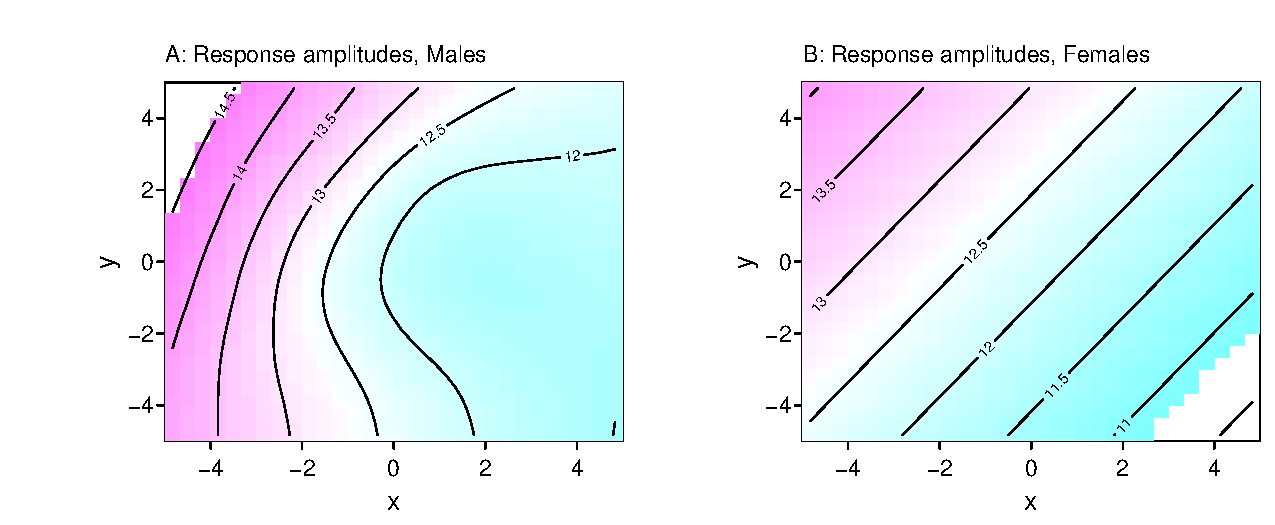
\includegraphics[width=0.97\textwidth]{figs/8-plotVIS-1} }

\end{Schunk}
\vspace*{-7pt}
\caption{Estimated contours of left eye responses to visual stimulae,
projected onto the plane.\label{fig:visAmp}}
\vspace*{15pt}
\end{figure*}
\end{fullwidth}
\enlargethispage{12pt}

The GAM fit will as far as possible use the smooth surface
to account for the pattern of variation across the eye, with
residuals from the surface treated as random normal noise.
\vspace*{7pt}

\begin{fullwidth}

\begin{Schunk}
\begin{Sinput}
## Code
library(DAAGviz)
library(mgcv)
eyeAmpM.gam <- gam(amp ~ s(x,y), data=subset(eyeAmp, Sex=="m"))
eyeAmpF.gam <- gam(amp ~ s(x,y), data=subset(eyeAmp, Sex=="f"))
lims <- range(c(predict(eyeAmpF.gam), predict(eyeAmpM.gam)))
vis.gam(eyeAmpM.gam, plot.type='contour', color="cm", zlim=lims, main="")
mtext(side=3, line=0.5, adj=0, "A: Response amplitudes, Males")
vis.gam(eyeAmpF.gam, plot.type='contour', color="cm", zlim=lims, main="")
mtext(side=3, line=0.5, adj=0, "B: Response amplitudes, Females")
\end{Sinput}
\end{Schunk}

\end{fullwidth}

\section{Other important models and issues}

\subsection{Errors in $x$}
In the classical "errors in $x$" model, one or more explanatory variables
are measured with error.  In straight line regression, the effect is to
attenuate the regression coefficient.  If there is, additionally, a
grouping factor with different means for the outcome variable for different
groups, a side effect of the attentuation is to make it appear that the
lines are different for the different groups.  The same general principles
apply when curves are fitted.  Where several variables
are measured with substantial error, there are increased oportunities for
transferring estimated effects between variables, and the mathematics
becomes more complicated.

Examples on the help page \txtt{?DAAG::errorsINx} show how to run
simulations that demonstrate the effects in the simple cases just
described.  These are useful in giving a sense of the magitutude
of the attenuation, and any possible
apparent group difference, that may arise from a given amount of
measurement error.

Comparison with data from a case where $x$ is measured with minimal 
error is needed, in order to get a data-based indication of the extent
of the error in $x$.

An alternative to the classical "errors in $x$" model is the Berkson
model.  Consider an oven where the strength of pottery fired in the
oven is a linear function, for some fixed time, of the temperature.  

\begin{itemize}
\item [-] For the classical "errors in $x$" model, the measured
temperature varies randomly about the oven temperature.
\item[-] For the Berkson model, the oven temperature varies randomly
about a temperature that is determined by setting on the temperature
control.
\end{itemize}

In the Berkson  case, the slope is an unbiased estimate of the true
slope, but has increased standard error.  In common situations, there
may be a mix of classical errors and Berkson, with some additional
bias.

\section{Exercises}
\begin{enumerate}
\item Exercise \ref{ex:mol1} in Section \ref{ss:wd} involved reading
  data into a data frame \txtt{molclock1}.  Plot \txtt{AvRate} against
  \txtt{Myr}. Fit a regression line (with intercept, or without
  intercept?), and add the regression line to the plot.  What
  interpretation can be placed upon the regression
  slope?\label{ex1:mod}

\item  Attach the \textit{DAAG} package. Type
\txtt{help(elasticband)} to see the help page for the data frame
\txtt{elasticband}.  Plot \txtt{distance} against
\txtt{stretch}. Regress \txtt{distance} against
\txtt{stretch} and explain how to interpret the coefficient.
\item Repeat the calculations in Section \ref{sec:nihills-reg}, now
examining the regression of \txtt{time} on \txtt{dist} and \txtt{climb}.
Does this regression adequately model the data. Comment on the results.
\item
\begin{enumerate}
\item Investigate the pairwise relationships between variables in the
data frame \txtt{oddbooks} ({\em DAAG}).
\item Fit the models
  \begin{fullwidth}
\begin{Schunk}
\begin{Sinput}
volume <- apply(oddbooks[, 1:3], 1, prod)
area <- apply(oddbooks[, 2:3], 1, prod)
lob1.lm <- lm(log(weight) ~ log(volume), data=oddbooks)
lob2.lm <- lm(log(weight) ~ log(thick)+log(area), data=oddbooks)
lob3.lm <- lm(log(weight) ~ log(thick)+log(breadth)+log(height),
              data=oddbooks)
\end{Sinput}
\end{Schunk}
\end{fullwidth}
Comment on what you find, i.e., comment both on the estimates and on
the standard errors.
\item Can \txtt{weight} be completely explained as a function of
\txtt{volume}?  Is there another relevant variable?
\end{enumerate}
\item Repeat the calculations in Section \ref{sec:nihills}, now
  with the dataset \txtt{hills2000} (\textit{DAAG}).  Do any of
  the points stand out as outliers?  Use \txtt{predict()},
  with \txtt{newdata = hills200}, to obtain predictions from the
  \txtt{hills2000} model for the \txtt{nihills} data.  Compare with
  the predictions from the \txtt{nihills} model.

  %% \item In the data frame \txtt{molclock} of Exercise \ref{ex1:mod},
  %% data are estimates of amino acid replacements per 100 million years,
  %% for the three genes \txtt{GPDH}, \txtt{SOD}, and \txtt{XDH}. The
  %% column \txtt{Ave} is a weighted average of these three, with weights
  %% proportional to sequence length.  Use regression to determine the
  %% weights that were used.
\end{enumerate}
